\documentclass[]{IEEEtran}
% Your packages go here
\usepackage[utf8]{inputenc}
\usepackage{graphicx}
\usepackage{grffile}
\usepackage{gensymb}
\usepackage{amsmath}
\usepackage{amssymb}
\usepackage{listings}
\usepackage{mathtools}
\usepackage{subfig}
\usepackage{xcolor}
\usepackage{multirow}
\usepackage{xfrac}
\usepackage{amsmath}
\usepackage{float}
\DeclareMathOperator{\atantwo}{atan2}

\DeclareMathOperator{\arctantwo}{arctan2}


\definecolor{codegreen}{rgb}{0,0.6,0}
\definecolor{codegray}{rgb}{0.5,0.5,0.5}
\definecolor{codepurple}{rgb}{0.58,0,0.82}
\definecolor{backcolour}{rgb}{0.95,0.95,0.92}

\lstdefinestyle{mystyle}{
    backgroundcolor=\color{backcolour},   
    commentstyle=\color{codegreen},
    keywordstyle=\color{magenta},
    numberstyle=\tiny\color{codegray},
    stringstyle=\color{codepurple},
    basicstyle=\ttfamily\footnotesize,
    breakatwhitespace=false,         
    breaklines=true,                 
    captionpos=b,                    
    keepspaces=true,                 
    numbers=left,                    
    numbersep=5pt,                  
    showspaces=false,                
    showstringspaces=false,
    showtabs=false,                  
    tabsize=2
}
 
\lstset{style=mystyle}
 
\usepackage{lipsum}% http://ctan.org/pkg/lipsum
\usepackage{graphicx}% http://ctan.org/pkg/graphicx

\def\footnoterule{\relax%
  \kern-2pt
  \hbox to \columnwidth{\hfill\vrule width 0.7\columnwidth height 0.4pt\hfill}
  \kern4.6pt}
\makeatother

\renewcommand{\lstlistingname}{Algorithm}% Listing -> Algorithm
\usepackage[noadjust]{cite}
\markboth{MO435 - Probabilistic Machine Learning }{}

% \usepackage{graphicx}
% \graphicspath{{../output/}}

\begin{document}

\title{Project 2}
\author{Ivan Lima do Espirito Santo \thanks{RA: 956694 - i956694@g.unicamp.br}\\ Rosa Yuliana Gabriela Paccotacya Yanque \thanks{RA: 263068 - r263068@dac.unicamp.br} \\ Thiago Gomes Marçal Pereira \thanks{RA: 189691 - t189691@g.unicamp.br}}




\maketitle
  
% \begin{abstract}
% \end{abstract}
  
\section{Introduction} \label{sec:introduction}
A Gaussian process is a generalization of the Gaussian probability distribution. A Gaussian distribution in its general form is a function governed by stochastic properties (mean and covariance). We can understand this function as a infinity long vector, each entry in the vector specifies the function value \( f(x)\) at a particular input \(x\). If we ask only for the properties of the function at a finite number of points, then inference in the Gaussian process will give you the same answer if you ignore the infinitely many other points, as if you would have taken them all into account!~\cite{Ras2006}\par\( \)
In this project we implement a Gaussian Process and explore its accuracy regarding the number of training points and the choice of different Kernels and their parameters.


\section{Gaussian Processes}
\subsection{Overview}
In supervised learning, we observe some inputs~\({ x }_{ i }\) and some outputs~\({ y }_{ i }\). First, we assume that~\({ y }_{ i }=f({ x }_{ i })\), for some unknown function \(f\). Second, we infer a distribution over functions given the data,~\( p(f|X,y)\). Finally, we use this distribution to make predictions given new inputs, i.e., we compute:
\begin{equation}
p({ y }_{ * }|\mathbf{{ x }_{ * }},\mathbf{X},\mathbf{y})=\int { p({ y }_{ * }|{ f},\mathbf{{ x }_{ * }}) } p(f|\mathbf{X},\mathbf{y})df
\label{eq01}
\end{equation}

We can work with the function \(f\) in Equation~\ref{eq01} in its parametric representation, thus instead of inferring \(p(f|D)\), we infer \( p(\theta|D)\). Alternatively, Gaussian Process performs Bayesian inference over functions themselves, i.e.~\(p(f|D)\), in a non-parametric sense that is not worrying how many parameters are involved since there could be an infinite number of them. \par

Gaussian process,normally abbreviated as GP, defines a \textbf{prior over functions}, which can be converted into a \textbf{posterior over functions} once we have seen some data. We only need to be able to define a distribution over the function’s values at a finite, but \textbf{arbitrary}, set of points, say~\({{x}_1,...,{x}_N}\). A GP assumes that~\({p(f({x}_1),...,f({x}_N))}\)  is \textbf{jointly Gaussian}, with some mean~\(\mathbf{\mu (x)}\) and covariance~\(\mathbf{\Sigma (x)}\) given by~\({ \Sigma  }_{ ij }={ \kappa (x }_{ i },{ x }_{ j })\), where~\(\kappa\) is a positive definite kernel function that measures similarity (see Appendix~\ref{sec:appendix-1} for more information about kernels). The key idea is that if \(\mathbf{{x}_i}\) and \(\mathbf{{x}_j}\) are deemed by the kernel to be similar, then we expect the output of the function at those points to be similar. See~\cite{Ras2006} for detailed explanations.

\subsection{GPs for regression}
Let the prior on the regression function be a GP, denoted by:
\begin{equation}
f(x)\sim GP(m(x),\kappa (x, x' ))
\label{eq02}
\end{equation}
where~\(m(x)\) is the mean function and~\(\kappa (x, x')\)  is the kernel or covariance function, defined by:
\begin{equation}
m(x)\quad =\quad \mathbb{E} (f(x))
\label{eq03}
\end{equation}
\begin{equation}
\kappa (x,\acute { x } )={ \mathbb{E}[ }(f(x)-m(x))({ f(\acute { x } )-m(\acute { x } ) })^{ T }]
\label{eq04}
\end{equation}
We require~\(\kappa (.)\) to be a positive definite kernel. So, for any finite set of points, this process defines a joint Gaussian:
\begin{equation}
p(\mathbf{f}|{ \mathbf{X} })=\mathcal{N} (\mathbf{f}|\mu ,\mathbf{\mathrm{K}} )
\label{eq05}
\end{equation}
where~\({ \mathrm{K}  }_{ ij }={ \kappa (x }_{ i },{ x }_{ j })\) and~\(\mu =(m({ x }_{ 1 }),...,m({ x }_{ N }))\)

\subsection{Predictions using noise-free observations }
Suppose we observe a noise-free training data where~\({ f }_{ i }=f({ x }_{ i })\) is the noiseless observation of the function evaluated at~\({ x }_{ i }\). Given a test data~\({ X }_{ * }\) of size~\({ N }_{ * } \times D\), we want to predict the function outputs~\({ f }_{ * }\). GP works as an \textbf{interpolator} of the training data. The joint distribution has the following form: (see~\cite{Mur2012} chapter 4 for detailed explanation on Gaussian properties)
\begin{equation}
\begin{pmatrix} f \\ { f }_{ * } \end{pmatrix}\sim \mathcal{N} \left( \begin{pmatrix} \mu  \\ { \mu  }_{ * } \end{pmatrix},\begin{pmatrix} \mathrm{K}  & { \mathrm{K}  }_{ * } \\ { \mathrm{K}  }_{ * }^{ T } & { \mathrm{K}  }_{ ** } \end{pmatrix} \right) 
\label{eqM15p6}
\end{equation}
From the  Gaussian conditioning rules (~\cite{Bar2010} definition 78), the \textbf{posterior} has the form:

\begin{equation}
p({ f }_{ * }|{ X }_{ * },X,f)=\mathcal{N}({ f }_{ * }|{ \mu  }_{ * },{ \Sigma  }_{ * })
\label{eq15p9A}
\end{equation}

\begin{equation}
{ \mu  }_{ * }=\mu ({ X }_{ * })+{ \mathrm{K}  }_{ * }^{ T }{ \mathrm{K}  }^{ -1 }(f-\mu (X))
\label{eq15p9B}
\end{equation}

\begin{equation}
{ \Sigma  }_{ * }={ \mathrm{K}  }_{ ** }{ -{ \mathrm{K}  }_{ * }^{ T }\mathrm{K}  }^{ -1 }{ \mathrm{K}  }_{ * })
\label{eq15p9C}
\end{equation}

If we use  squared exponential kernel, it assumes the form:
\begin{equation}
\kappa (x,\acute { x } )={ \sigma  }_{ f }^{ 2 }exp(-\frac { 1 }{ 2{ \ell  }^{ 2 } } { (x-\acute { x) }  }^{ 2 })
\label{M15p10}
\end{equation}
\subsection{Predictions using noisy observations  }
In this case, the function assumes the form~\(y=f({ x })+\epsilon \), where~\(\epsilon \sim \mathcal{N}(0,{ \sigma  }_{ y }^{ 2 })\). The covariance of the observed noise response is:
\begin{equation}
cov\left[ y|X \right] =\mathrm{K}+{ \sigma  }_{ y }^{ 2 }{ \mathrm{I}  }_{ N }={\mathrm{K} }_{ y }
\label{M15p12}
\end{equation}
where the matrix is diagonal due to the assumption that the noise terms are independently added to each observation. The joint density of the observed data is then:
\begin{equation}
\begin{pmatrix} y \\ { f }_{ * } \end{pmatrix}\sim { N }\left( 0,\begin{pmatrix} { { \mathrm{K} }_{ y } } & { { \mathrm{K} } }_{ * } \\ { { \mathrm{K} } }_{ * }^{ T } & { {\mathrm{K} } }_{ ** } \end{pmatrix} \right) 
\label{M15p13}
\end{equation}
and the \textbf{posterior predictive density} assumes the form:
\begin{equation}
p({ f }_{ * }|{ X }_{ * },X,f)={ \mathcal{N} }({ f }_{ * }|{ \mu  }_{ * },{ \Sigma  }_{ * })
\label{M15p17A}
\end{equation}

\begin{equation}
{ \mu  }_{ * }=\mu ({ X }_{ * })+{ { \mathrm{K} } }_{ * }^{ T }{ { {\mathrm{K} }_{ y }^{ -1 } } }y)
\label{M15p17B}
\end{equation}

\begin{equation}
{ \Sigma  }_{ * }={ { \mathrm{K} } }_{ ** }{ -{ { \mathrm{K} } }_{ * }^{ T } }{ \mathrm{K} }_{ y }^{ -1 }{ { \mathrm{K} } }_{ * })
\label{M15p17C}
\end{equation}
We can write the posterior mean in another way, as follows:
\begin{equation}
\bar { { f }_{ * } } = { \mathrm{K} }_{ * }^{ T }{ \mathrm{K} }_{ y }^{ -1 }y=\sum _{ i=1 }^{ N }{ { \alpha  }_{ i }\kappa ({ x }_{ i },{ x }_{ * }) } 
\label{M15p18}
\end{equation}
where~\(\alpha ={ K }_{ y }^{ -1 }y\).
More on the posterior predictive density on section~\ref{imple}.
\subsection{Effect of the kernel parameters }
To illustrate the influence of the kernel parameter on the prediction, suppose we choose the  squared-exponential (SE) kernel for the noisy observations, as following:
\begin{equation}
{ \kappa  }_{ y }({ x }_{ p },{ x }_{ q })={ \sigma  }_{ f }^{ 2 }exp(-\frac { 1 }{ 2{ \ell  }^{ 2 } } { { ({ x }_{ p }-{ x }_{ q } }) }^{ 2 })+{ \sigma  }_{ y }^{ 2 }{ \delta  }_{ pq }
\label{M15p19}
\end{equation}
Note that~\(\ell\) is the horizontal scale over which the function changes,~\({ \sigma  }_{ f }^{ 2 }\) controls the vertical scale of the function, and~\({ \sigma  }_{ y }^{ 2 }\) is the noise variance.
\subsection{Estimating the kernel parameters   }
Considering an empirical Bayes approach and  maximizing the marginal likelihood, which in log has the following form:

\begin{multline}
log(p(y|{ X }))= \\
={ log(\mathcal{N} }(y|0,{ \mathrm{K} }_{ y })) \\
=-\frac { 1 }{ 2 } y{ \mathrm{K} }_{ y }^{ -1 }y-\frac { 1 }{ 2 } log\left| { \mathrm{K} }_{ y } \right| -\frac { N }{ 2 } log(2\pi )
\label{M15p22}
\end{multline}

The first term is a data fit term, the second term is a model complexity term, and the third term is just a constant. Now denoting the kernel hyper parameters by~\(\theta \), we have: 
\begin{multline}
\frac { \partial  }{ { \partial \theta  }_{ j } } log(p(y|{ X }))= \\
=\frac { 1 }{ 2 } { y }^{ T }{ { \mathrm{K} } }_{ y }^{ -1 }\frac { \partial { \mathrm{K} }_{ y } }{ { \partial \theta  }_{ j } } { { \mathrm{K} } }_{ y }^{ -1 }y-\frac { 1 }{ 2 } tr({ { \mathrm{K} } }_{ y }^{ -1 }\frac { \partial { \mathrm{K} }_{ y } }{ { \partial \theta  }_{ j } } )
\label{M15p23}
\end{multline}

\begin{equation}
\frac { \partial  }{ { \partial \theta  }_{ j } } log(p(y|{ X }))=\frac { 1 }{ 2 } tr(({ { \alpha { \alpha  }^{ T }-\mathrm{K} } }_{ y }^{ -1 })\frac { \partial { \mathrm{K} }_{ y } }{ { \partial \theta  }_{ j } } )
\label{M15p24}
\end{equation}
where~\({ { \alpha =K } }_{ y }^{ -1 }y\). One can note from equations~\ref{M15p23} and~\ref{M15p24} that the partial derivative depends on the form of the kernel. Given an expression for the log \textbf{marginal likelihood} and its \textbf{derivative}, we can estimate the kernel parameters using any standard \textbf{gradient-based optimizer}.\par
An alternative to computing a point estimate of the hyper-parameters is to compute their posterior via Bayesian inference for the hyper-parameters. More on that in~\cite{Mur2012}, section 15.2.4.2. Also, one can use a quite different approach to optimize kernel parameters known as \textbf{multiple kernel learning}. See~\cite{Mur2012}, section 15.2.4.3 for more details.

\subsection{Computational and numerical approach}
The predictive mean depends on a matrix inversion. For reasons of numerical stability, it is unwise to directly invert it.  A more robust alternative is to compute a Cholesky decomposition. \par
Summarizing, the six steps sequence for the GP approach is as follows:
\begin{enumerate}
    \item \(\mathbf{L=cholesky(K+{ \sigma  }_{ y }^{ 2 }I)}\)
    \item \(\mathbf{\alpha ={ L }^{ T }\setminus (L\setminus y)}\)
    \item \(\mathbf{E[{ f }_{ * }]={ K }_{ * }^{ T }\alpha}\)
    \item \(\mathbf{V=L\setminus { \kappa  }_{ * }}\)
    \item \(\mathbf{var[{ f }_{ * }]=\kappa ({ x }_{ * },{ x }_{ * })-{ v }^{ T }v}\)
    \item \(\mathbf{logp(y|{ X }) = -\frac { 1 }{ 2 } { y }^{ T }\alpha  -{\Sigma  }_{ i }log{ L }_{ ii}-\frac { N }{ 2 } log(2\pi )}\)
\end{enumerate}

Cholesky decomposition is a way to solve a linear system that works as follows:\par
~\(A x = b\)\par
~\(A={ L }^{ T }L\) once~\(A\) is a positive defined matrix, we have:\par
~\({ L }^{ T }[Lx]=b\)\par
~\({ L }^{ T }\theta=b \), solve for ~\(\theta\).\par
~\(Lx=\theta\), solve for ~\(x\).\par

\section{Project Description}
In this project we implemented a Bayesian Optimization procedure using Gaussian Processes(GPs). We encapsulate the behavior of the GPs in a class that can be instantiated as follows:

\begin{verbatim}
gp = GP(kernel, sigma) 
gp.addData(xtrain, ytrain) 
mu, s2 = gp.posterior(xtest)
\end{verbatim}

where GP is the class we created, kernel is any kernel function, and, sigma is the prior of the noise’s standard deviation. Thus, our implementation encapsulates the Bayesian Optimization process in a single class.

\section{Implementation}
\label{imple}
Given an~\((n,d)\)-array of data $x$  and an n-vector of corresponding $f(x)$, our Python code predicts the distribution of the~\((m,d)\) array of test data $x_*$.
%Given an~\((n,d)\)-array of data xtrain and an n-vector ytrain, our python code predict the distribution of the~\((m,d)\) array of test data xtest.
In order to do so, we compute the predictive posterior parameters~\(\mu \) and~\(\Sigma \) of the distribution function. They are the mean and the covariance, respectively. Our default kernel function is the widely known squared-exponential. For the one-dimensional case it is defined as: 
\begin{equation}
{ \kappa  }_{ \alpha  }({ x },\acute { x } )={ \sigma  }^{ 2 }exp\left( -\frac { { { ({ x }-\acute { x }  }) }^{ 2 } }{ 2{ \ell  }^{ 2 } }  \right) 
\label{p1}
\end{equation}

where~\( \alpha =(\sigma ,\ell )\) is the vector of hyperparameters, and~\(x\) and~\(\acute { x }\) are the data points used in the kernel, where the covariance matrix entries are~\({ K }_{ ij }={ k }_{ \alpha  }\left( { x }_{ i },{ x }_{ j } \right) \). In general, the kernel receives two arrays of size~\((n,d)\) and~\((m,d)\) and returns an~\((n,m)\)-array of all the pairwise evaluations. The kernel signature is: kernel~\((x1, x2, ell=1.0, s =1.0)\), where the parameters are optional. \par
Note that parameter ell is ~\(\ell\) and s is the ~\(\sigma\) in equation~\ref{p1}. We also call s as ~\({\sigma}_{f}\) to differentiate from the noise variance ~\({\sigma}_{y}\); 
~\(\ell\) is the horizontal scale over which the function ~\({ \sigma  }_{ f }^{ 2 }\) changes. 
As already said, we have the following Gaussian joint distribution:

\begin{equation}
\begin{pmatrix} f \\ { f }_{ * } \end{pmatrix}\sim \mathcal{N} \left( \begin{pmatrix} \mu  \\ { \mu  }_{ * } \end{pmatrix},\begin{pmatrix} \mathrm{K}  & { \mathrm{K}  }_{ * } \\ { \mathrm{K}  }_{ * }^{ T } & { \mathrm{K}  }_{ ** } \end{pmatrix} \right) 
\label{eqM15p6_02}
\end{equation}


We derive the posterior function by using the properties of a joint and condition distribution of a MVN. Equation 4.68 of~\cite{Mur2012}. The proof of  the theorem stated in this equation requires inverse of a partitioned matrix using Schur complements and the matrix inversion lemma. One can find the entire algebraic steps in section 4.3.4 of~\cite{Mur2012}  

Therefore, we implement the posterior function as stated in equations~\ref{eq15p9A},~\ref{eq15p9B}, and~\ref{eq15p9C}.

\section{Experiments and Discussions}~\(\)
For our experiments we create a data set for training (seed 42) and testing (seed 33).
%we defined two fixed seeds for each data set so we can have the same results every time the code is executed. 
For our 1D tests we use sine, square and cubic functions with SE kernel (square exponential). We sample 5,10,50 points from each of them to define our train points. We repeat this very same process for Rational, Ornstein, and Gamma Kernel. For Rational Kernel we use \(\alpha = 0.5\), and for Gamma Kernel we use \(\gamma = 0.2\) for all the experiments. See Appendix~\ref{sec:appendix-1} for Kernels definition.

\subsection{Different Amount of Data}
To observe the behavior of the learned function, we plot the mean plus minus two standard deviations to see the variation (uncertainty) of the predicted functions.\par 
Figure~\ref{SE_sin} shows the results for 5, 10, and 50 number of points with and without noise for SE kernel and sin function. The shaded area represents the expectation of \(f(x)\pm 2std(f(x))\) One can see from the behavior that for 5 points the shape of the curve resembles a sin function with zero uncertainty in the 5 points. For points other than training points, the uncertainty is high. \par
As we increase the number of points, the curve tends to a sin in the region of the data training points. For other regions the uncertainty is still pretty high. In other words, we have a very good prediction on the training points region. From Figure~\ref{SE_sin_noise}, we see that the noise prevents perfect fit even in the training points due to the uncertainty caused by the prior noise. However, despite the noise, it's still a good prediction.  

\begin{figure}[h]
  \centering
  \subfloat[5 points]{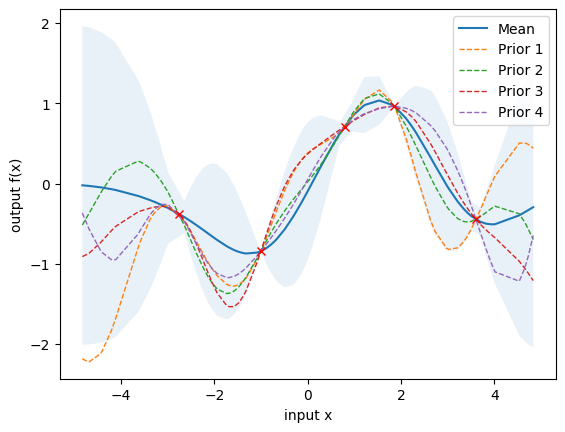
\includegraphics[width=0.238\textwidth]{images/1D_5points_SE_Kernel_sin_noiseless.png}}
  \hspace{1mm}
    \subfloat[10 points]{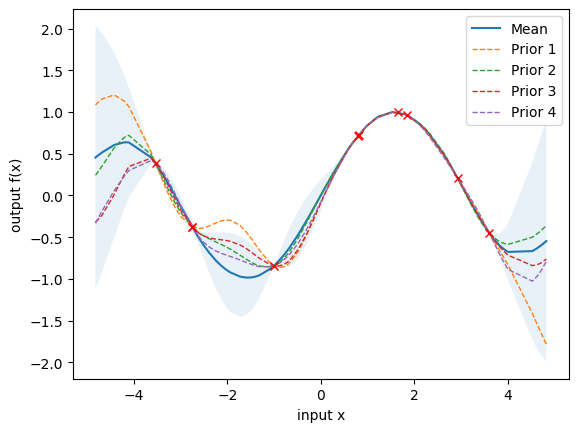
\includegraphics[width=0.238\textwidth]{images/1D_10points_SE_Kernel_sin_noiseless.png}}
  \hspace{1mm}
   \subfloat[50 points]{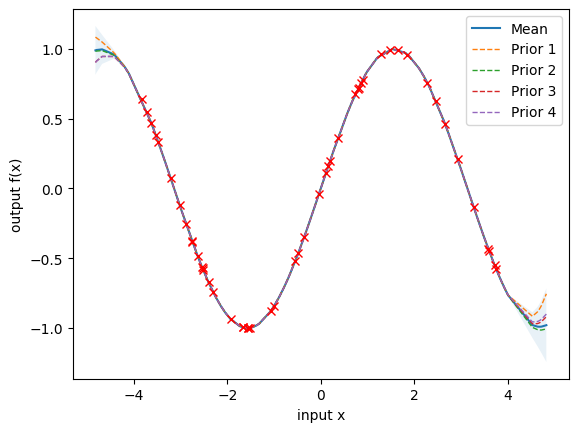
\includegraphics[width=0.26\textwidth]{images/1D_50points_SE_Kernel_sin_noiseless.png}}
  \hspace{1mm}
  
  \caption{Square Exponential Kernel for a noise-free sin function.}
  \label{SE_sin}
\end{figure}\par
  
  
\begin{figure}[h]
  \centering
  \subfloat[5 points]{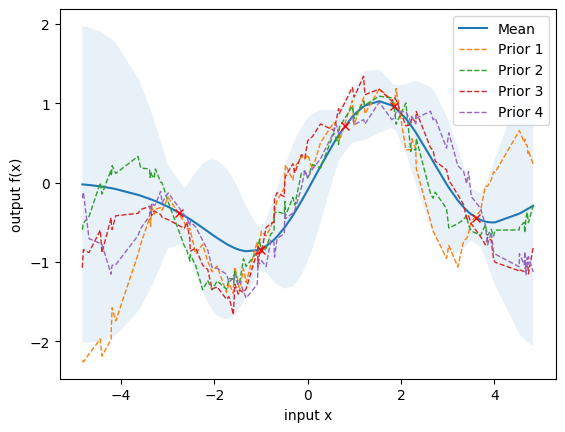
\includegraphics[width=0.238\textwidth]{images/1D_5points_SE_Kernel_sin_noise.png}}
  \hspace{1mm}
    \subfloat[10 points]{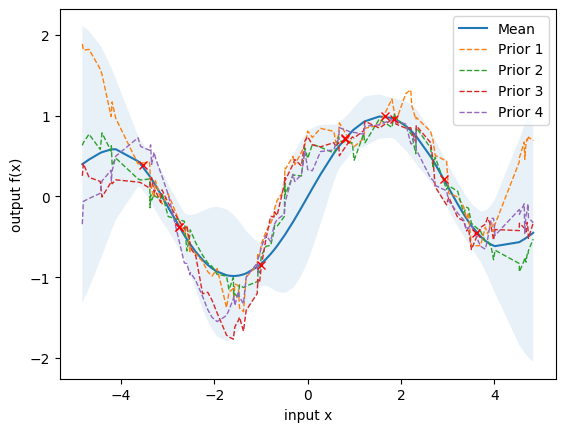
\includegraphics[width=0.238\textwidth]{images/1D_10points_SE_Kernel_sin_noise.png}}
  \hspace{1mm}
   \subfloat[50 points]{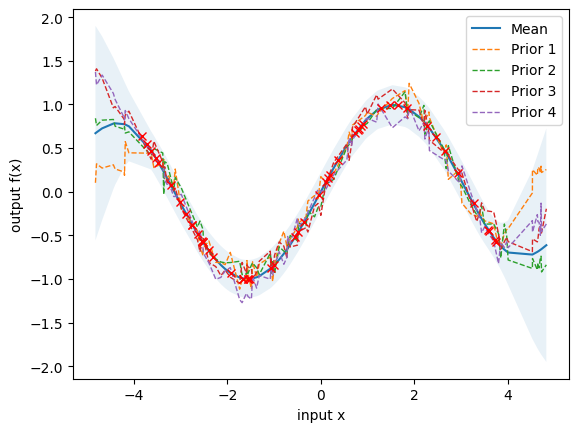
\includegraphics[width=0.26\textwidth]{images/1D_50points_SE_Kernel_sin_noise.png}}
  \hspace{1mm}
  
  \caption{Square Exponential Kernel for a noise (0.1) sin function.}
  \label{SE_sin_noise}
\end{figure}\par

We observe the same behavior for other functions and kernels. See Appendix~\ref{sec:appendix-2} for Rational, Ornstein, and Gamma Kernels and square and cubic functions.

\subsection{Higher Dimensional Data}
Our implementation is general enough to evaluate higher dimensional data. The results for 2D data is shown in Figures~\ref{2D_SE_sin}.
We observe a increase in accuracy as the number of training points gets higher.  
\begin{figure}[H]
  \centering
  \subfloat[5 points]{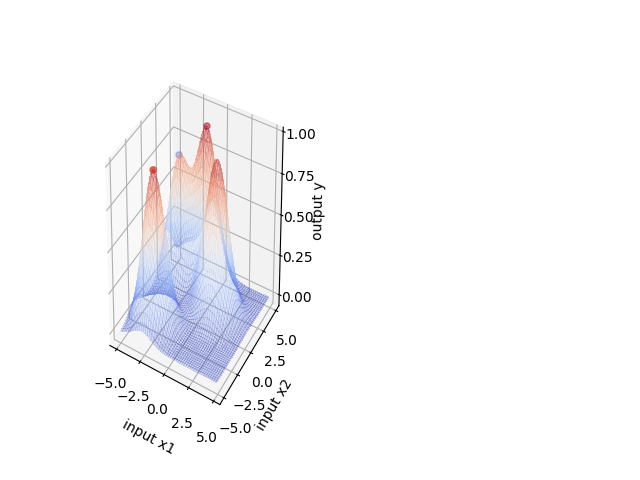
\includegraphics[trim={0.5cm 0.5cm 7cm 1cm},clip,width=0.23\textwidth]{images/2D_5points_SE_Kernel_sin_noiseless.png}}
  \hspace{1mm}
    \subfloat[10 points]{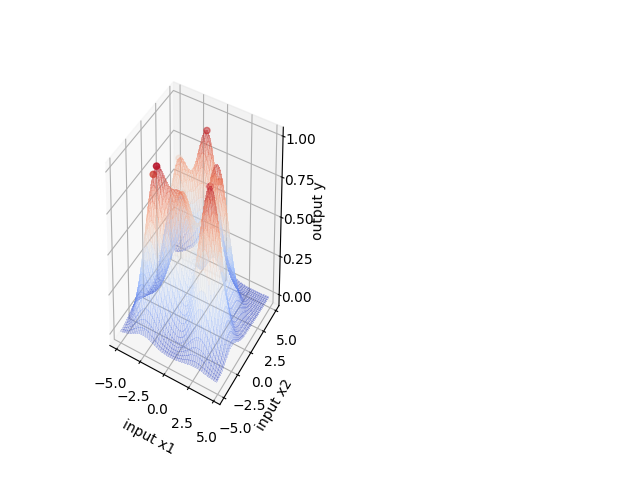
\includegraphics[trim={0.5cm 0.5cm 7cm 1cm},clip,width=0.23\textwidth]{images/2D_10points_SE_Kernel_sin_noiseless.png}}
  \hspace{1mm}
   \subfloat[50 points]{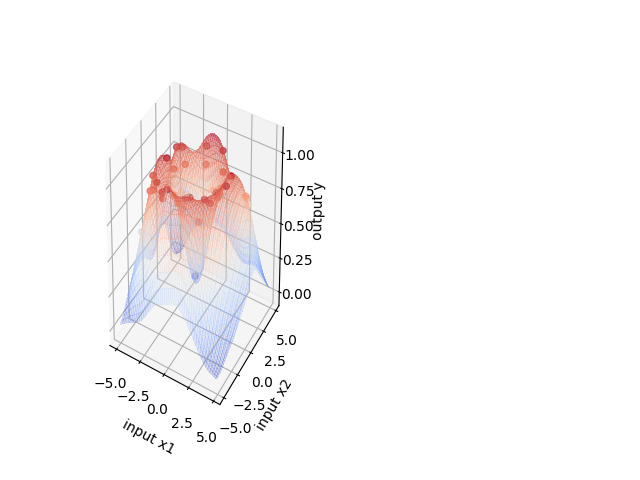
\includegraphics[trim={0.5cm 0.5cm 7cm 1cm},clip,width=0.23\textwidth]{images/2D_50points_SE_Kernel_sin_noiseless.png}}
  \hspace{1mm}
  
  \subfloat[5 points]{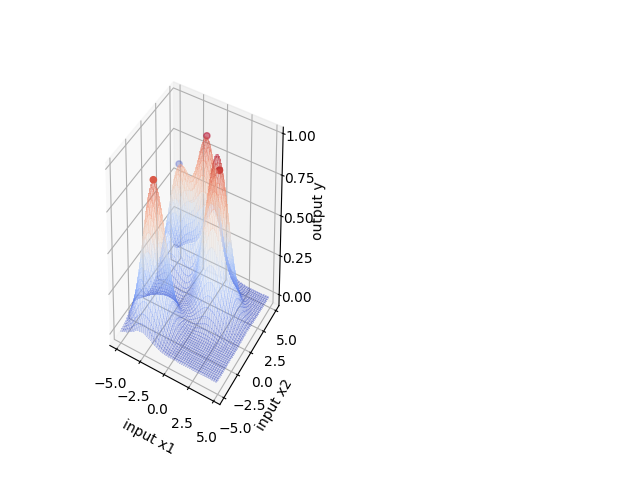
\includegraphics[trim={0.5cm 0.5cm 7cm 1cm},clip,width=0.23\textwidth]{images/2D_5points_SE_Kernel_sin_noise.png}}
  \hspace{1mm}
    \subfloat[10 points]{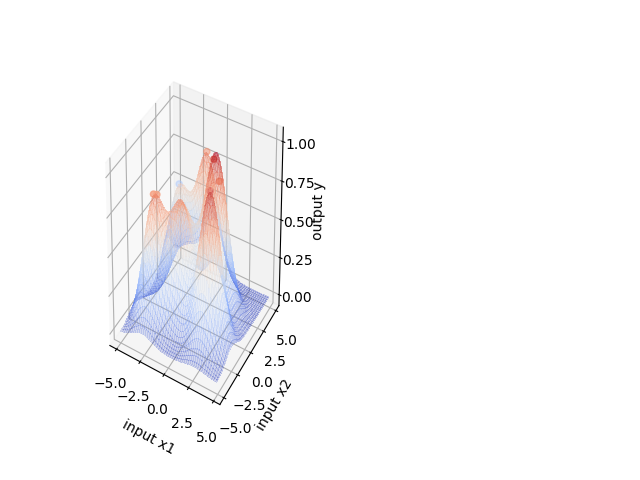
\includegraphics[trim={0.5cm 0.5cm 7cm 1cm},clip,width=0.23\textwidth]{images/2D_10points_SE_Kernel_sin_noise.png}}
  \hspace{1mm}
   \subfloat[50 points]{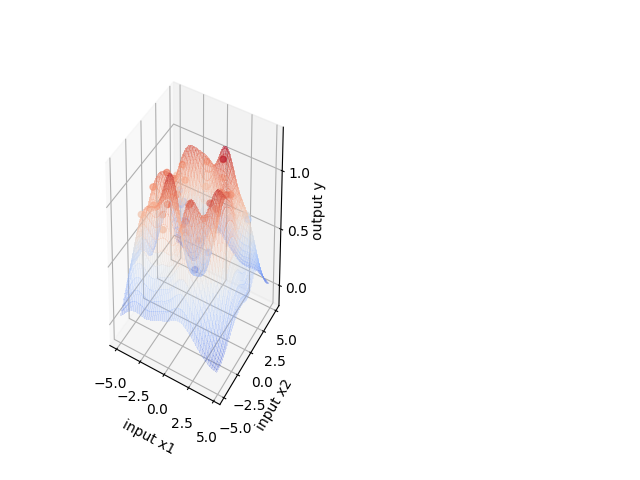
\includegraphics[trim={0.5cm 0.5cm 7cm 1cm},clip,width=0.23\textwidth]{images/2D_50points_SE_Kernel_sin_noise.png}}
  \hspace{1mm}
  
  \caption{Square Exponential Kernel for a sin function (a),(b), and (c) noise-free, and (d), (e), and (f) with 0.1 noise variance with 2D input data}
  \label{2D_SE_sin}
\end{figure}\par



\subsection{Effect of Kernel Parameters}
To understand the influence of the kernel parameters on the prediction, we performed experiments choosing the  squared-exponential (SE) kernel for a noisy observations havin in min the Equation~\ref{M15p19_}.
\begin{equation}
{ \kappa  }_{ y }({ x }_{ p },{ x }_{ q })={ \sigma  }_{ f }^{ 2 }exp(-\frac { 1 }{ 2{ \ell  }^{ 2 } } { { ({ x }_{ p }-{ x }_{ q } }) }^{ 2 })+{ \sigma  }_{ y }^{ 2 }{ \delta  }_{ pq }
\label{M15p19_}
\end{equation}

Note that~\(\ell\) is the horizontal scale over which the function changes,~\({ \sigma  }_{ f }^{ 2 }\) controls the vertical scale of the function, and~\({ \sigma  }_{ y }^{ 2 }\) is the noise variance.\par

To illustrate how the kernel parameters influence on the prediction we run experiments with different combination of them. The parameters were chosen according table~\ref{parametros}.

\begin{table}[!h]
\centering
\begin{tabular}{|c|c|c|c|c|}
\hline
\textbf{parameters}                  &         & (a)       & (b)       & (c)       \\ \hline
horizontal scale                     & \(\ell\) & 1.0 & 0.3 & 3.0 \\ \hline
vertical scale                       & \({ \sigma  }_{ f }^{ 2 }\) & 1.0 & 1.08 & 1.16 \\ \hline
\multicolumn{1}{|l|}{noise variance} & \({ \sigma  }_{ y }^{ 2 }\) & 0.1 & 0.00005 & 0.89 \\ \hline
\end{tabular}
\caption{Set of parameters for experiments }
\label{parametros}
\end{table}

Figure~\ref{SE_sin_hyper} shows the results with 50 training points.

\begin{figure}[!h]
  \centering
  \subfloat[]{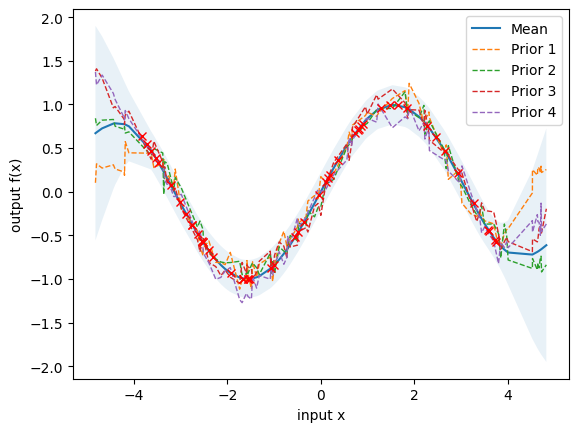
\includegraphics[width=0.238\textwidth]{images/1D_50points_SE_Kernel_sin_noiseless_A_params.png}}
  \hspace{1mm}
    \subfloat[]{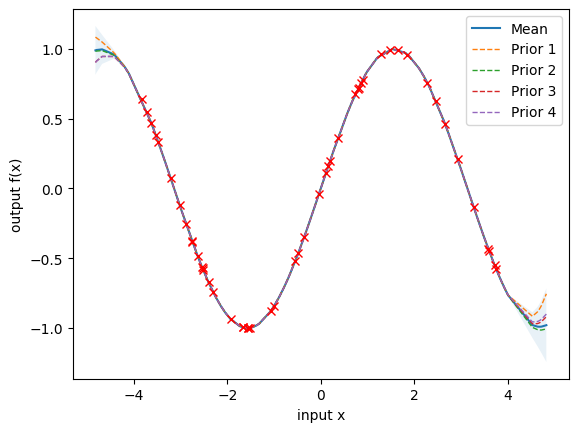
\includegraphics[width=0.238\textwidth]{images/1D_50points_SE_Kernel_sin_noiseless_B_params.png}}
  \hspace{1mm}
   \subfloat[]{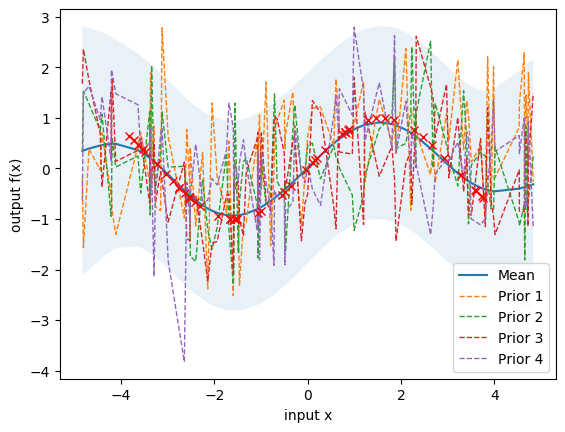
\includegraphics[width=0.238\textwidth]{images/1D_50points_SE_Kernel_sin_noiseless_C_params.png}}
  \hspace{1mm}
  \caption{Square Exponential Kernel for different set of parameters according to the  table~\ref{parametros}.}
  \label{SE_sin_hyper}
\end{figure}\par

The results in (a) are a good fit. At (b) the function looks smoother. At experiment (c), the function looks more “wiggly” and  the uncertainty goes up faster, since the effective distance from the training points increases more rapidly. \par

We can find the optimal parameter by minimizing the negative log marginal likelihood with respect to the parameter (equation~\ref{M15p22}).The parameter optimization is shown on  Table~\ref{optimization}.

\begin{table}[!h]
\centering
\begin{tabular}{|c|c|c|c|c|c|}
\hline
& Exp. 1&Exp. 2 &Exp. 3& Exp. 4 & Exp. 5\\ \hline
initial ell    & 1.0     & 0.5     & 2.0     & 2.0     & 3.0     \\ \hline
initial  s  & 1.0     & 1.0     & 2.0     & 5.0     & 4.0     \\ \hline
optimal  ell  & 3.01    & 2.75    & 2.82    & 3.15    & 2.91    \\ \hline
optimal  s  & 3.68    & 2.28    & 2.61    & 4.42    & 3.0     \\ \hline
likelihood & -136.89 & -137.06 & -137.11 & -136.63 & -137.09 \\ \hline
\end{tabular}
\caption{Initial and optimal values of parameters in different experiments  }
\label{optimization}
\end{table}\par

We see from the results that if we minimize directly from equation~\ref{M15p22}, the optimization does not work correctly due the complexity of the marginal likelihood function. A better option would have been to use equation~\ref{M15p24}  with a \textbf{gradient-based optimizer}. Moreover, implement it along with Cholesky decomposition to make it more stable. Note that the gradient depends on with respect to which parameter we derive partially. Therefore, the gradient depends on the Kernel type as well.
If we fix one parameter and calculate the marginal likelihood as a function of only one of them, we can have an idea of their optimal value. See Figure~\ref{like_vs_ell_s_noise}

\begin{figure}[!ht]
  \centering
  \subfloat[Likelihood vs ell]{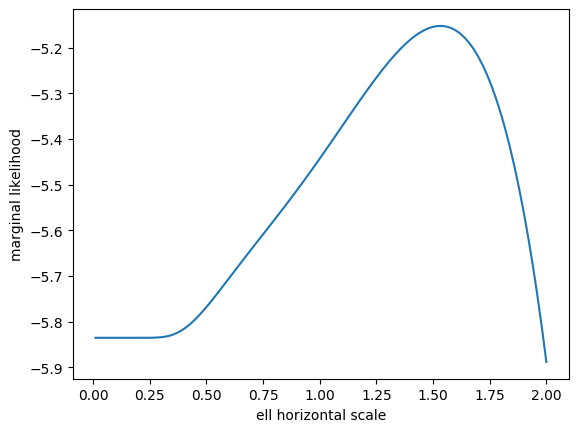
\includegraphics[width=0.238\textwidth]{images/1D_SE_Kernel_sin_likelihood_vs_ell}}
  \hspace{1mm}
  \subfloat[Likelihood vs s]{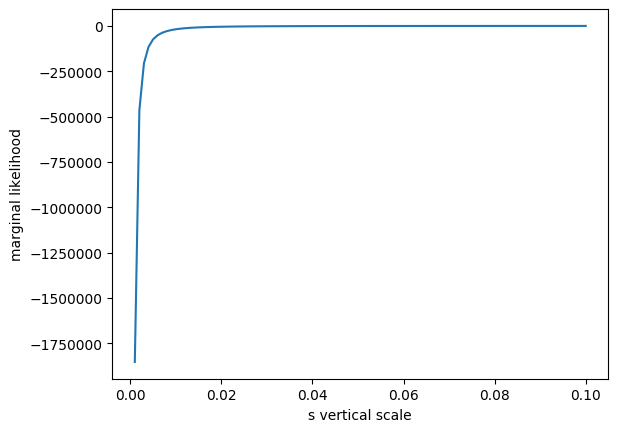
\includegraphics[width=0.238\textwidth]{images/1D_R_Kernel_sin_likelihood_vs_s.png}}
  \hspace{1mm}
  \subfloat[Likelihood vs noise]{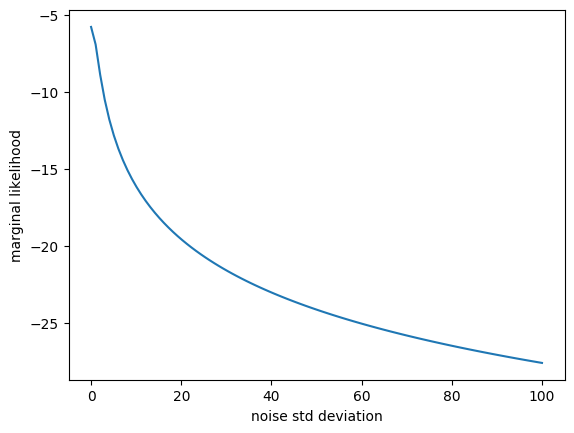
\includegraphics[width=0.238\textwidth]{images/1D_O_Kernel_sin_likelihood_vs_noise}}
  \hspace{1mm}
 \caption{Likelihood vs horizontal scale ell.}
  \label{like_vs_ell_s_noise}
\end{figure}\par

Note from Figure~\ref{like_vs_ell_s_noise} (a) that the~\(\ell\) optimal occurs about~\(1.6\) when fixing \({ \sigma  }_{ f }^{ 2 }=s=1.0\) and \({ \sigma  }_{ y }^{ 2 }=noise=0.00005\). 

From Figure~\ref{like_vs_ell_s_noise} (b), fixing ~\(\ell=1.0\) and \({ \sigma  }_{ y }^{ 2 }=noise=0.00005\), the \({ \sigma  }_{ f }^{ 2 }=s\) too small affects negatively the likelihood, but only up to a certain value when its increase has minor impact on the likelihood. 
Finally, from Figure~\ref{like_vs_ell_s_noise} (c), fixing ~\(\ell=1.0\) and \({ \sigma  }_{ f }^{ 2 }=s=1.0\), as the variance of noise increases, the uncertainty increases too, as expected. 
See the Appendix~\ref{sec:appendix-5} for the results using others Kernels.\par
Another way to visualize the parameter influence on the prediction is to plot the contour of the negative marginal likelihood at some parameter combination. See Figure~\ref{contour_plots}


\begin{figure}[!htb]
  \centering
  \subfloat[ell vs noise]{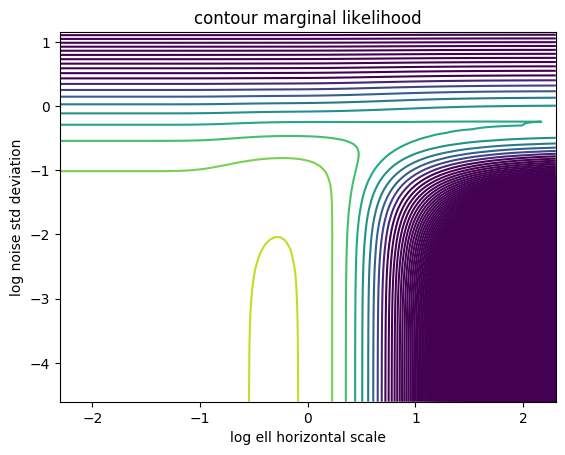
\includegraphics[width=0.238\textwidth]{images/1D_O_Kernel_sin_contour_noise_vs_ell_log.png}}
  \hspace{1mm}
  \subfloat[ell vs s]{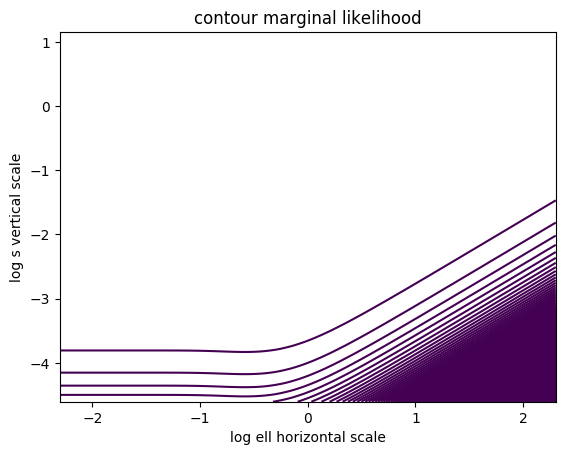
\includegraphics[width=0.238\textwidth]{images/1D_O_Kernel_sin_contour_s_vs_ell_log.png}}
  \hspace{1mm}
  \caption{Likelihood contour plots for Ornstein Kernel and sin function.}
  \label{contour_plots}
\end{figure}\par
See Appendix~\ref{sec:appendix-6} for contour plots with other Kernels.\par

Also, the equation~\ref{M15p19_} can be generalized for higher dimension cases by introducing a term M in equation:
\begin{equation}
{ \kappa  }_{ y }({ x }_{ p },{ x }_{ q })={ \sigma  }_{ f }^{ 2 }exp(-\frac { 1 }{ 2{ \ell  }^{ 2 } } { { ({ x }_{ p }-{ x }_{ q } }) }^{ T }M{ ({ x }_{ p }-{ x }_{ q } }))+{ \sigma  }_{ y }^{ 2 }{ \delta  }_{ pq }
\label{M15p19b}
\end{equation}\par
 So, we can run experiments in the same way  with the elements of the M matrix to understand the influence they have on the prediction. 
 
\subsection{Effect of Kernel}
The Kernel defines the variance function between the points. It is by definition symmetric positively defined. See Appendix~\ref{sec:appendix-1} for different Kernel definitions.\par
Figures~\ref{Kernels_cubic} and~\ref{Kernels} show the same experiment with four different Kernels with 5 and 50 training points respectively. 


\begin{figure}[!htb]
  \centering
  \subfloat[SE Kernel]{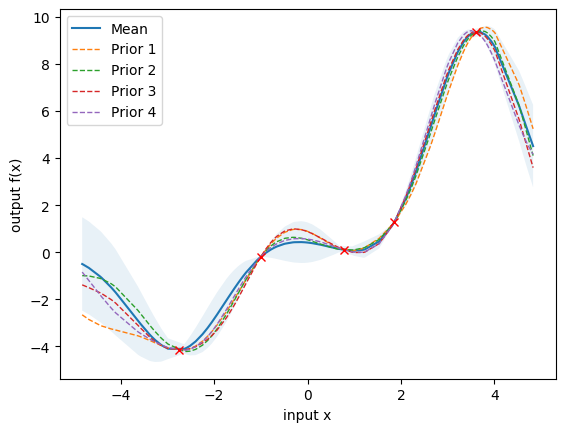
\includegraphics[width=0.238\textwidth]{images/1D_5points_SE_Kernel_cubic_noiseless.png}}
  \hspace{1mm}
    \subfloat[Rational Kernel]{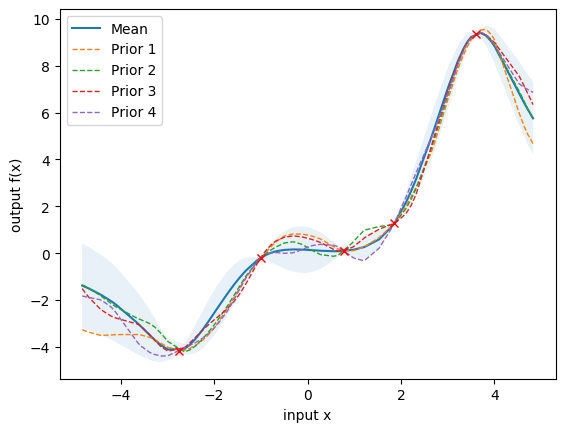
\includegraphics[width=0.238\textwidth]{images/1D_5points_Rational_Kernel_cubic_noiseless.png}}
  \hspace{1mm}
   \subfloat[Ornstein Kernel]{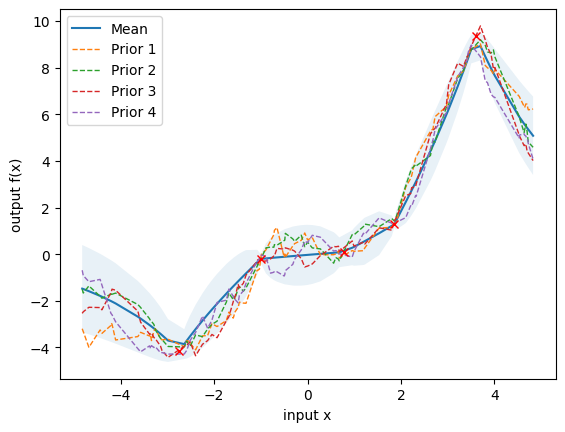
\includegraphics[width=0.238\textwidth]{images/1D_5points_Ornstein_Kernel_cubic_noiseless.png}}
  \hspace{1mm}
  \subfloat[Gamma Kernel]{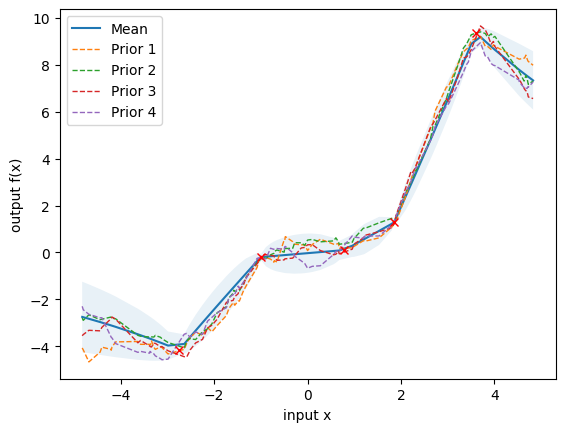
\includegraphics[width=0.238\textwidth]{images/1D_5points_Gamma_Kernel_cubic_noiseless.png}}
  \hspace{1mm}
  \caption{Experiment with 4 different Kernels using a cubic function with 5 training points.}
  \label{Kernels_cubic}
\end{figure}\par


\begin{figure}[!ht]
  \centering
  \subfloat[SE Kernel]{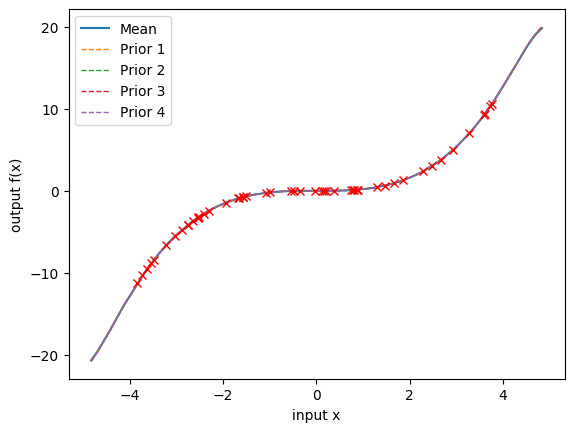
\includegraphics[width=0.238\textwidth]{images/1D_50points_SE_Kernel_cubic_noiseless.png}}
  \hspace{1mm}
    \subfloat[Rational Kernel]{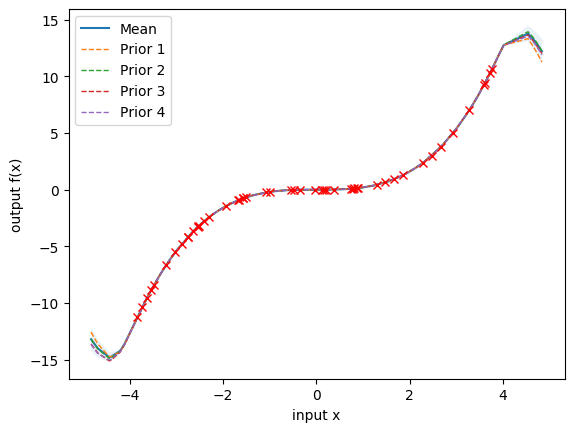
\includegraphics[width=0.238\textwidth]{images/1D_50points_Rational_Kernel_cubic_noiseless.png}}
  \hspace{1mm}
   \subfloat[Ornstein Kernel]{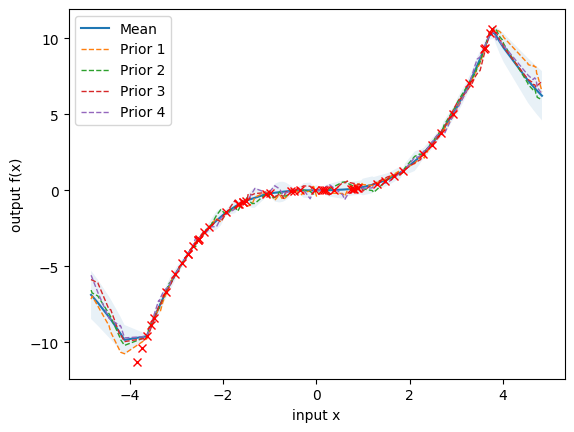
\includegraphics[width=0.238\textwidth]{images/1D_50points_Ornstein_Kernel_cubic_noiseless.png}}
  \hspace{1mm}
  \subfloat[Gamma Kernel]{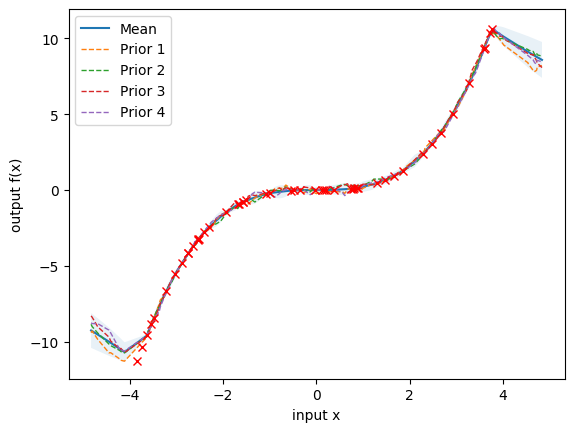
\includegraphics[width=0.238\textwidth]{images/1D_50points_Gamma_Kernel_cubic_noiseless.png}}
  \hspace{1mm}
  \caption{Experiment with 4 different Kernels using a cubic function with 50 training points.}
  \label{Kernels}
\end{figure}\par
Note that some Kernels work better with a low number of training points, however, all of them provide a good fit with more data points.

\section{Conclusions}
We implemented a Gaussian Process for regression and explore the different behaviors of learned functions, kernels and hyper-parameters.

The simple idea of finding a distribution over possible functions that are consistent with the observed data, combined with the Bayesian approach that updates the prior as more data is observed and generating posterior distribution over functions, proved to be extremely powerful. It can be understood as a generalization of other techniques with the advantages of the straight forward implementation for both regression and classification problems.

Although the accuracy of the predictions is closely related to the number of data training points, we achieve reasonable efficiency with a relatively low amount. Regarding the variance function defined by the Kernel, we can choose them from a variety of types and tuning its parameter to attend our predictions requirements of time and accuracy. 

As a lesson learnt, the Cholesky decomposition to avoid matrix inversion proved to be the preferable implementation to gain computational speed and avoid numerical instability. Furthermore, with respect to hyper-parameters optimization, we realized that using the negative marginal likelihood in its log form and applying a python minimization built-in method to find the optimal kernel parameter should be avoided.  Instead, we should implement the partial derivatives with respect to each hyper-parameter and use a gradient-based optimizer. 

\bibliographystyle{abbrv}
\bibliography{bibliography}






\clearpage
\onecolumn
\begin{appendices}

\section{Covariance function} \label{sec:appendix-1}
 Defination of Covariance function: Given any collection of points \({x}^{1},...,{x}^{M}\), a covariance function  \(k({x}_{i},{x}_{j})\) defines the elements of a \(M\times M\) matrix: 
\begin{equation}
\left[ { C }_{ ij } \right] =k({ x }_{ i },{ x }_{ j })
\label{kernel00}
\end{equation}
such that \(C\) is positive semidefinite.\par
\subsection{Stationary Kernel}
 A kernel  \({\kappa  }({ x },\acute { x } )\) is stationary if the kernel depends only on the separation \({ { ({ x }-\acute { x }  }) }\). That is 
\begin{equation}
{ \kappa  }({ x },\acute { x } )={ \kappa  }{ { ({ x }-\acute { x }  }) }
\label{kernel01}
\end{equation}\par
\subsubsection{Squared Exponential}
\begin{equation}
{ \kappa  }(d)={ e }^{ -{ \left| d \right|  }^{ 2 } }
\label{kernel02}
\end{equation}
where \({d} = { ({ x }-\acute { x }  })\)\par
\subsubsection{\(\gamma\)-Exponential}
\begin{equation}
{ \kappa  }(d)={ e }^{ -{ \left| d \right|  }^{ \gamma  } }\quad ,0<\lambda \le 2
\label{kernel03}
\end{equation}\par
\subsubsection{Mat\'ern}
\begin{equation}
{ \kappa  }(d)={ \left| d \right|  }^{ { \nu  } }{ K }_{ \nu  }\left( \left| d \right|  \right) 
\label{kernel04}
\end{equation}
where \({ K }_{ \nu  }\) is a modified Bessel function, \(\nu >0\).\par
\subsubsection{Rational Quadratic}
\begin{equation}
{ \kappa  }(d)={ \left( 1+{ \left| d \right|  }^{ 2 } \right)  }^{ -\alpha  }\quad,  \alpha >0
\label{kernel05}
\end{equation}\par
\subsubsection{ Periodic}
For 1-dimensional \(x\) and \(\acute { x }\), a stationary (and isotropic) covariance function can be obtained by first mapping \(x\) to the two dimensional vector \(u(x) = (cos(x),sin(x))\) and then using the SE covariance \({ e }^{ -{ \left( u(x)-u(\acute { x) }  \right)  }^{ 2 } }\)
\begin{equation}
k(x-\acute { x } )={ e }^{ -\lambda { sin }^{ 2 }(\omega (x-\acute { x } )) }\quad ,\lambda >0
\label{kernel06}
\end{equation}



\newpage
\section{Experimenting in 1 Dimension - Changing Kernel, input size and function } \label{sec:appendix-2} 

\begin{figure}[!ht]
  \centering
  \subfloat[5 points]{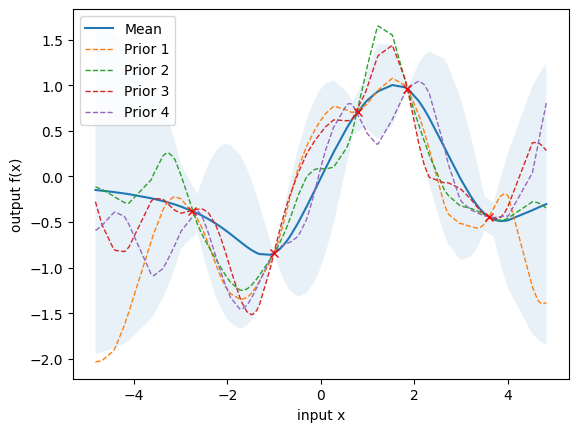
\includegraphics[width=0.29\textwidth]{images/1D_5points_Rational_Kernel_sin_noiseless.png}}
  \hspace{1mm}
    \subfloat[10 points]{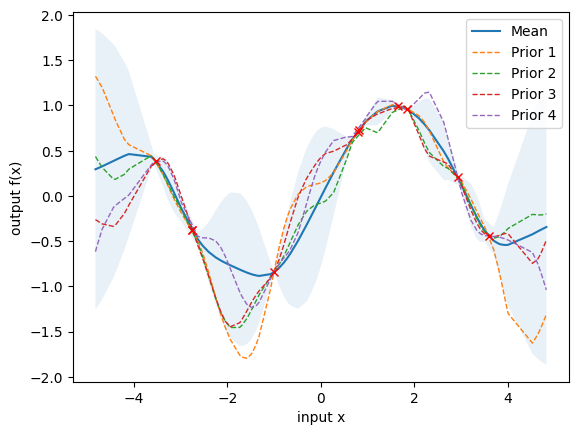
\includegraphics[width=0.29\textwidth]{images/1D_10points_Rational_Kernel_sin_noiseless.png}}
  \hspace{1mm}
   \subfloat[50 points]{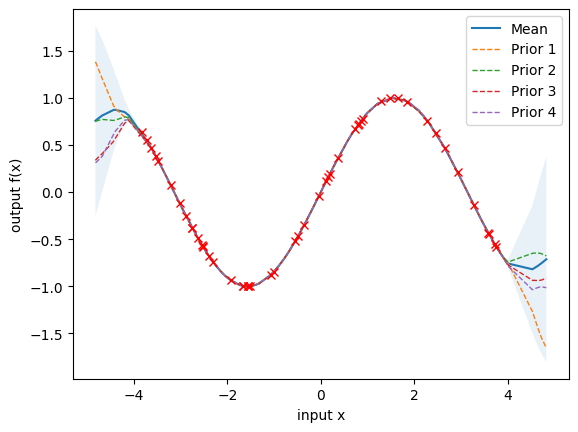
\includegraphics[width=0.29\textwidth]{images/1D_50points_Rational_Kernel_sin_noiseless.png}}
  \hspace{1mm}
  
  \subfloat[5 points]{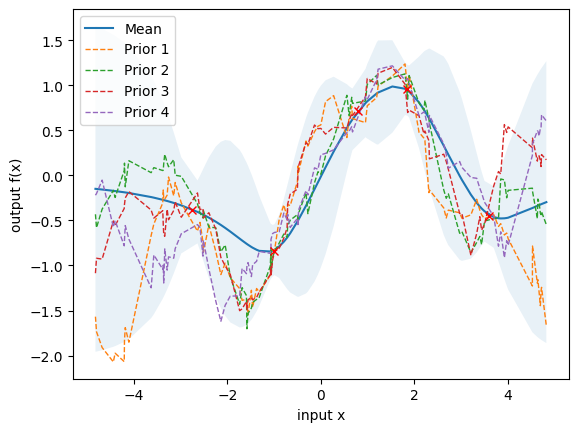
\includegraphics[width=0.29\textwidth]{images/1D_5points_Rational_Kernel_sin_noise.png}}
  \hspace{1mm}
    \subfloat[10 points]{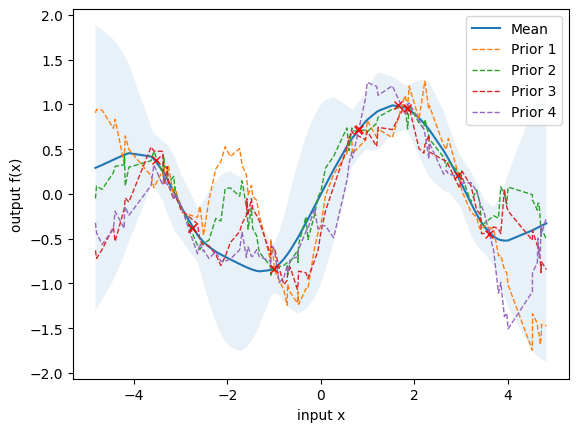
\includegraphics[width=0.29\textwidth]{images/1D_10points_Rational_Kernel_sin_noise.png}}
  \hspace{1mm}
   \subfloat[50 points]{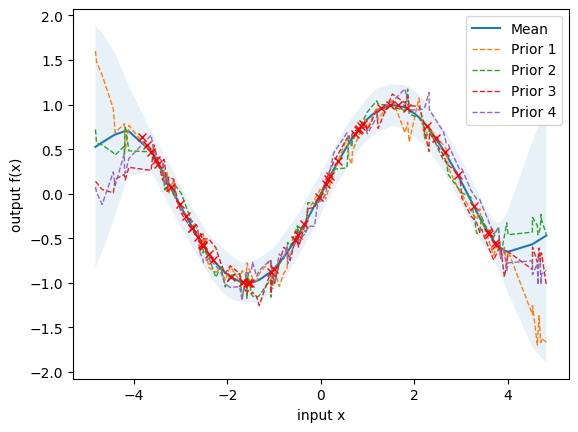
\includegraphics[width=0.29\textwidth]{images/1D_50points_Rational_Kernel_sin_noise.png}}
  \hspace{1mm}
  
  \caption{Rational Kernel (\(\alpha = 0.5\)) for a sin function.}
  \label{Rational_sin}
\end{figure}\par

\begin{figure}[!ht]
  \centering
  \subfloat[5 points]{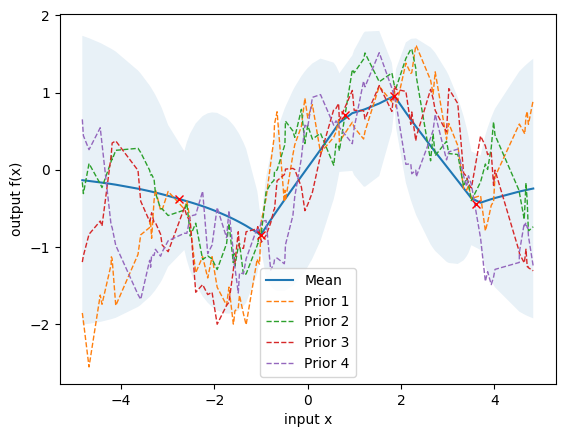
\includegraphics[width=0.29\textwidth]{images/1D_5points_Ornstein_Kernel_sin_noiseless.png}}
  \hspace{1mm}
    \subfloat[10 points]{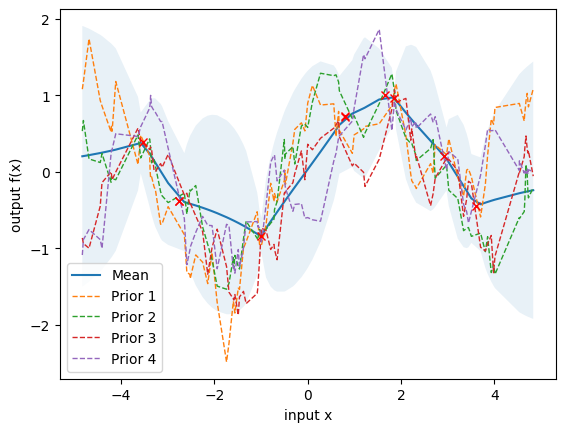
\includegraphics[width=0.29\textwidth]{images/1D_10points_Ornstein_Kernel_sin_noiseless.png}}
  \hspace{1mm}
   \subfloat[50 points]{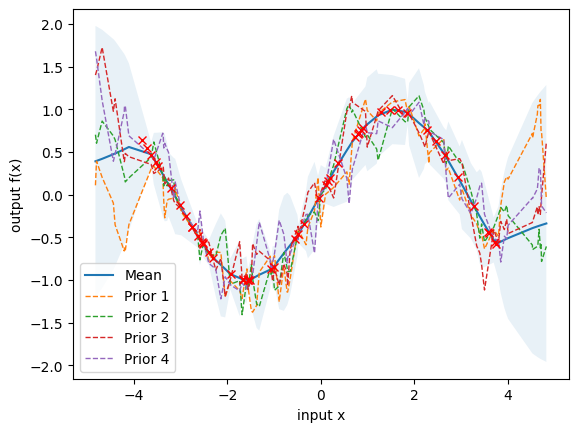
\includegraphics[width=0.29\textwidth]{images/1D_50points_Ornstein_Kernel_sin_noiseless.png}}
  \hspace{1mm}
  
  \subfloat[5 points]{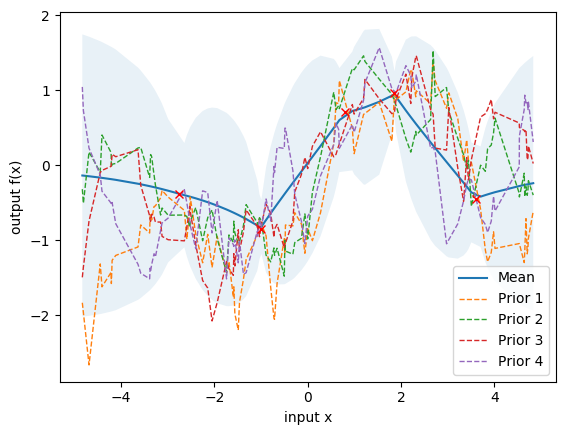
\includegraphics[width=0.29\textwidth]{images/1D_5points_Ornstein_Kernel_sin_noise.png}}
  \hspace{1mm}
    \subfloat[10 points]{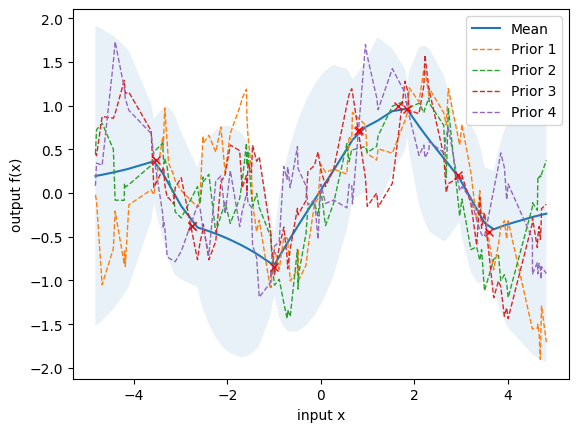
\includegraphics[width=0.29\textwidth]{images/1D_10points_Ornstein_Kernel_sin_noise.png}}
  \hspace{1mm}
   \subfloat[50 points]{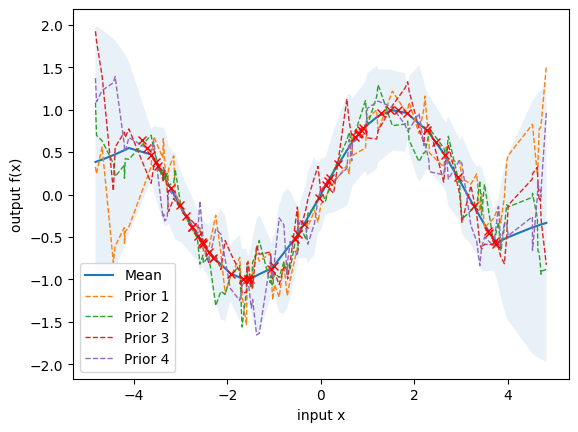
\includegraphics[width=0.29\textwidth]{images/1D_50points_Ornstein_Kernel_sin_noise.png}}
  \hspace{1mm}
  
  \caption{Ornstein Kernel for a sin function.}
  \label{Ornstein_sin}
\end{figure}\par

\begin{figure}[!ht]
  \centering
  \subfloat[5 points]{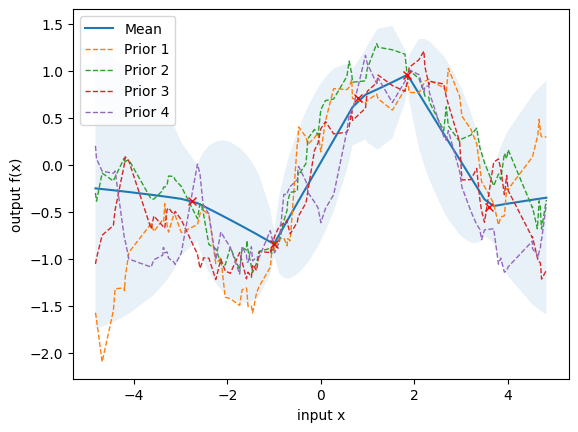
\includegraphics[width=0.29\textwidth]{images/1D_5points_Gamma_Kernel_sin_noiseless.png}}
  \hspace{1mm}
    \subfloat[10 points]{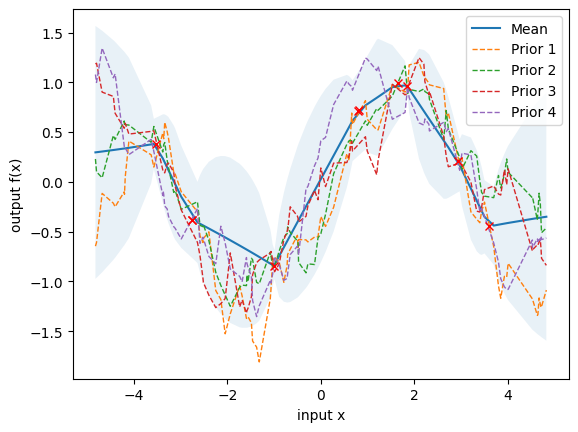
\includegraphics[width=0.29\textwidth]{images/1D_10points_Gamma_Kernel_sin_noiseless.png}}
  \hspace{1mm}
   \subfloat[50 points]{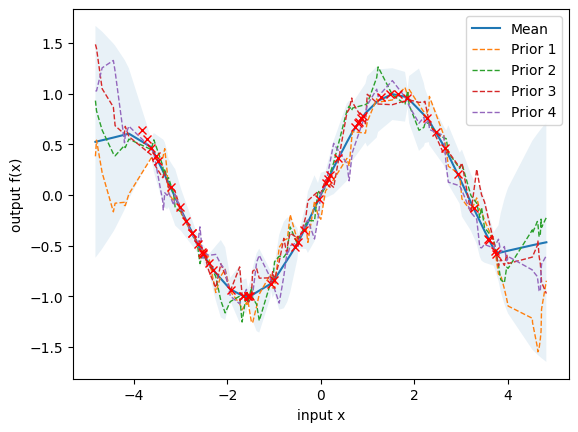
\includegraphics[width=0.29\textwidth]{images/1D_50points_Gamma_Kernel_sin_noiseless.png}}
  \hspace{1mm}
  
  \subfloat[5 points]{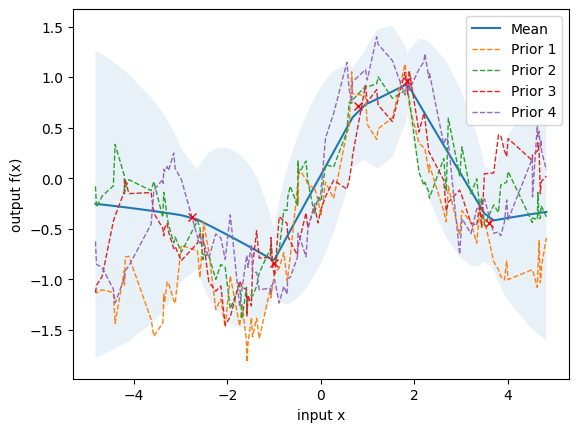
\includegraphics[width=0.29\textwidth]{images/1D_5points_Gamma_Kernel_sin_noise.png}}
  \hspace{1mm}
    \subfloat[10 points]{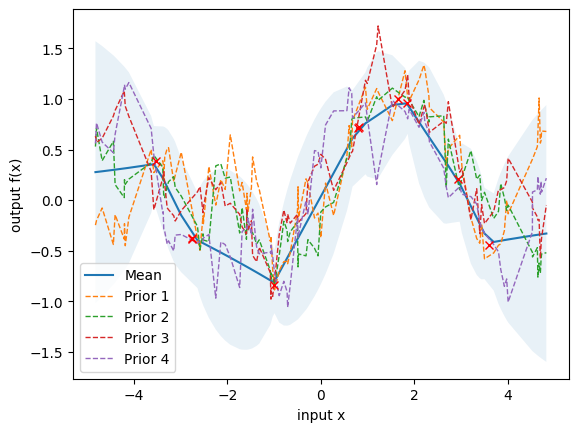
\includegraphics[width=0.29\textwidth]{images/1D_10points_Gamma_Kernel_sin_noise.png}}
  \hspace{1mm}
   \subfloat[50 points]{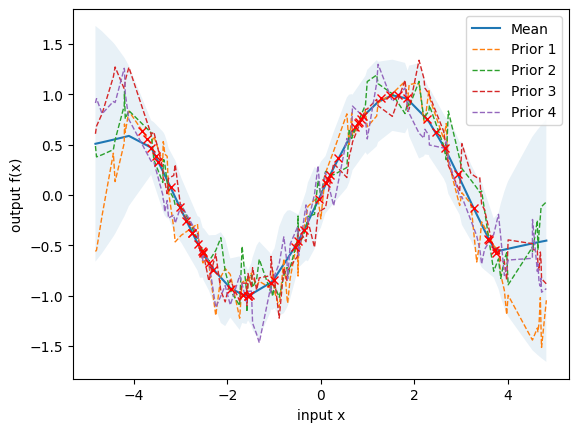
\includegraphics[width=0.29\textwidth]{images/1D_50points_Gamma_Kernel_sin_noise.png}}
  \hspace{1mm}
  
  \caption{Gamma Kernel (\(\gamma = 0.2\)) for a sin function.}
  \label{Gamma_sin}
\end{figure}\par
\begin{figure}[!ht]
  \centering
  \subfloat[5 points]{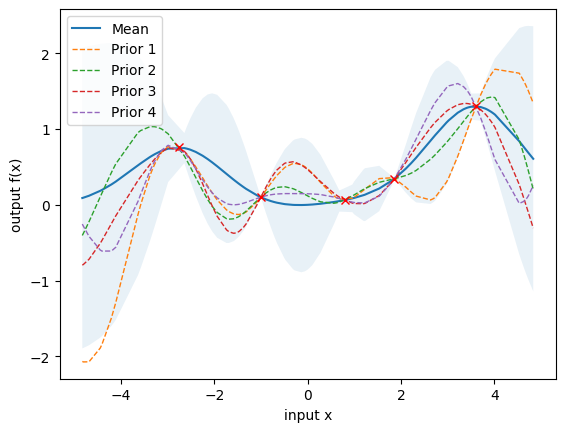
\includegraphics[width=0.29\textwidth]{images/1D_5points_SE_Kernel_square_noiseless.png}}
  \hspace{1mm}
    \subfloat[10 points]{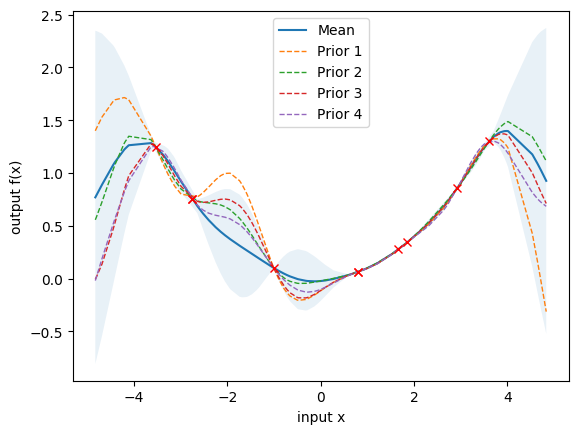
\includegraphics[width=0.29\textwidth]{images/1D_10points_SE_Kernel_square_noiseless.png}}
  \hspace{1mm}
   \subfloat[50 points]{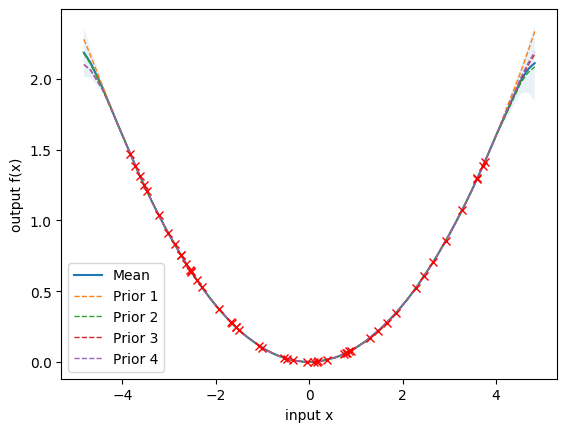
\includegraphics[width=0.29\textwidth]{images/1D_50points_SE_Kernel_square_noiseless.png}}
  \hspace{1mm}
  
  \subfloat[5 points]{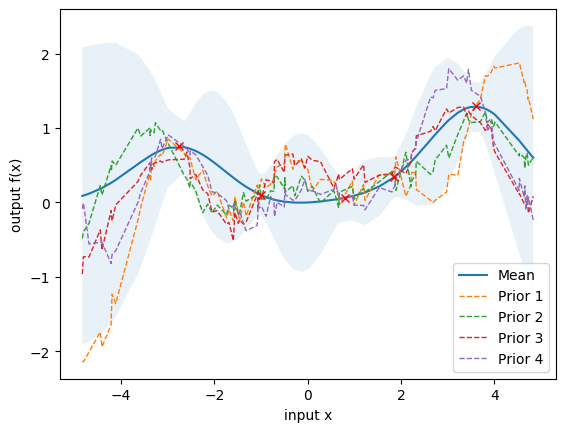
\includegraphics[width=0.29\textwidth]{images/1D_5points_SE_Kernel_square_noise.png}}
  \hspace{1mm}
    \subfloat[10 points]{\includegraphics[width=0.29\textwidth]{images/1D_10points_SE_Kernel_square_noise.png}}
  \hspace{1mm}
   \subfloat[50 points]{\includegraphics[width=0.29\textwidth]{images/1D_50points_SE_Kernel_square_noise.png}}
  \hspace{1mm}
  
  \caption{Square Exponential Kernel for a square function.}
  \label{SE_square}
\end{figure}\par

\begin{figure}[!ht]
  \centering
  \subfloat[5 points]{\includegraphics[width=0.29\textwidth]{images/1D_5points_Rational_Kernel_square_noiseless.png}}
  \hspace{1mm}
    \subfloat[10 points]{\includegraphics[width=0.29\textwidth]{images/1D_10points_Rational_Kernel_square_noiseless.png}}
  \hspace{1mm}
   \subfloat[50 points]{\includegraphics[width=0.29\textwidth]{images/1D_50points_Rational_Kernel_square_noiseless.png}}
  \hspace{1mm}
  
  \subfloat[5 points]{\includegraphics[width=0.29\textwidth]{images/1D_5points_Rational_Kernel_square_noise.png}}
  \hspace{1mm}
    \subfloat[10 points]{\includegraphics[width=0.29\textwidth]{images/1D_10points_Rational_Kernel_square_noise.png}}
  \hspace{1mm}
   \subfloat[50 points]{\includegraphics[width=0.29\textwidth]{images/1D_50points_Rational_Kernel_square_noise.png}}
  \hspace{1mm}
  
  \caption{Rational Kernel (\(\alpha = 0.5\)) for a square function.}
  \label{Rational_square}
\end{figure}\par

\begin{figure}[!ht]
  \centering
  \subfloat[5 points]{\includegraphics[width=0.29\textwidth]{images/1D_5points_Ornstein_Kernel_square_noiseless.png}}
  \hspace{1mm}
    \subfloat[10 points]{\includegraphics[width=0.29\textwidth]{images/1D_10points_Ornstein_Kernel_square_noiseless.png}}
  \hspace{1mm}
   \subfloat[50 points]{\includegraphics[width=0.29\textwidth]{images/1D_50points_Ornstein_Kernel_square_noiseless.png}}
  \hspace{1mm}
  
  \subfloat[5 points]{\includegraphics[width=0.29\textwidth]{images/1D_5points_Ornstein_Kernel_square_noise.png}}
  \hspace{1mm}
    \subfloat[10 points]{\includegraphics[width=0.29\textwidth]{images/1D_10points_Ornstein_Kernel_square_noise.png}}
  \hspace{1mm}
   \subfloat[50 points]{\includegraphics[width=0.29\textwidth]{images/1D_50points_Ornstein_Kernel_square_noise.png}}
  \hspace{1mm}
  
  \caption{Ornstein Kernel for a square function.}
  \label{Ornstein_square}
\end{figure}\par

\begin{figure}[!ht]
  \centering
  \subfloat[5 points]{\includegraphics[width=0.29\textwidth]{images/1D_5points_Gamma_Kernel_square_noiseless.png}}
  \hspace{1mm}
    \subfloat[10 points]{\includegraphics[width=0.29\textwidth]{images/1D_10points_Gamma_Kernel_square_noiseless.png}}
  \hspace{1mm}
   \subfloat[50 points]{\includegraphics[width=0.29\textwidth]{images/1D_50points_Gamma_Kernel_square_noiseless.png}}
  \hspace{1mm}
  
  \subfloat[5 points]{\includegraphics[width=0.29\textwidth]{images/1D_5points_Gamma_Kernel_square_noise.png}}
  \hspace{1mm}
    \subfloat[10 points]{\includegraphics[width=0.29\textwidth]{images/1D_10points_Gamma_Kernel_square_noise.png}}
  \hspace{1mm}
   \subfloat[50 points]{\includegraphics[width=0.29\textwidth]{images/1D_50points_Gamma_Kernel_square_noise.png}}
  \hspace{1mm}
  
  \caption{Gamma Kernel (\(\gamma = 0.2\)) for a square function.}
  \label{Gamma_square}
\end{figure}\par
\begin{figure}[!ht]
  \centering
  \subfloat[5 points]{\includegraphics[width=0.29\textwidth]{images/1D_5points_SE_Kernel_cubic_noiseless.png}}
  \hspace{1mm}
    \subfloat[10 points]{\includegraphics[width=0.29\textwidth]{images/1D_10points_SE_Kernel_cubic_noiseless.png}}
  \hspace{1mm}
   \subfloat[50 points]{\includegraphics[width=0.29\textwidth]{images/1D_50points_SE_Kernel_cubic_noiseless.png}}
  \hspace{1mm}
  
  \subfloat[5 points]{\includegraphics[width=0.29\textwidth]{images/1D_5points_SE_Kernel_cubic_noise.png}}
  \hspace{1mm}
    \subfloat[10 points]{\includegraphics[width=0.29\textwidth]{images/1D_10points_SE_Kernel_cubic_noise.png}}
  \hspace{1mm}
   \subfloat[50 points]{\includegraphics[width=0.29\textwidth]{images/1D_50points_SE_Kernel_cubic_noise.png}}
  \hspace{1mm}
  
  \caption{Square Exponential Kernel for a cubic function.}
  \label{SE_cubic}
\end{figure}\par

\begin{figure}[!ht]
  \centering
  \subfloat[5 points]{\includegraphics[width=0.29\textwidth]{images/1D_5points_Rational_Kernel_cubic_noiseless.png}}
  \hspace{1mm}
    \subfloat[10 points]{\includegraphics[width=0.29\textwidth]{images/1D_10points_Rational_Kernel_cubic_noiseless.png}}
  \hspace{1mm}
   \subfloat[50 points]{\includegraphics[width=0.29\textwidth]{images/1D_50points_Rational_Kernel_cubic_noiseless.png}}
  \hspace{1mm}
  
  \subfloat[5 points]{\includegraphics[width=0.29\textwidth]{images/1D_5points_Rational_Kernel_cubic_noise.png}}
  \hspace{1mm}
    \subfloat[10 points]{\includegraphics[width=0.29\textwidth]{images/1D_10points_Rational_Kernel_cubic_noise.png}}
  \hspace{1mm}
   \subfloat[50 points]{\includegraphics[width=0.29\textwidth]{images/1D_50points_Rational_Kernel_cubic_noise.png}}
  \hspace{1mm}
  
  \caption{Rational Kernel (\(\alpha = 0.5\)) for a cubic function.}
  \label{Rational_cubic}
\end{figure}\par

\begin{figure}[!ht]
  \centering
  \subfloat[5 points]{\includegraphics[width=0.29\textwidth]{images/1D_5points_Ornstein_Kernel_cubic_noiseless.png}}
  \hspace{1mm}
    \subfloat[10 points]{\includegraphics[width=0.29\textwidth]{images/1D_10points_Ornstein_Kernel_cubic_noiseless.png}}
  \hspace{1mm}
   \subfloat[50 points]{\includegraphics[width=0.29\textwidth]{images/1D_50points_Ornstein_Kernel_cubic_noiseless.png}}
  \hspace{1mm}
  
  \subfloat[5 points]{\includegraphics[width=0.29\textwidth]{images/1D_5points_Ornstein_Kernel_cubic_noise.png}}
  \hspace{1mm}
    \subfloat[10 points]{\includegraphics[width=0.29\textwidth]{images/1D_10points_Ornstein_Kernel_cubic_noise.png}}
  \hspace{1mm}
   \subfloat[50 points]{\includegraphics[width=0.29\textwidth]{images/1D_50points_Ornstein_Kernel_cubic_noise.png}}
  \hspace{1mm}
  
  \caption{Ornstein Kernel for a cubic function.}
  \label{Ornstein_cubic}
\end{figure}\par

\begin{figure}[!ht]
  \centering
  \subfloat[5 points]{\includegraphics[width=0.29\textwidth]{images/1D_5points_Gamma_Kernel_cubic_noiseless.png}}
  \hspace{1mm}
    \subfloat[10 points]{\includegraphics[width=0.29\textwidth]{images/1D_10points_Gamma_Kernel_cubic_noiseless.png}}
  \hspace{1mm}
   \subfloat[50 points]{\includegraphics[width=0.29\textwidth]{images/1D_50points_Gamma_Kernel_cubic_noiseless.png}}
  \hspace{1mm}
  
  \subfloat[5 points]{\includegraphics[width=0.29\textwidth]{images/1D_5points_Gamma_Kernel_cubic_noise.png}}
  \hspace{1mm}
    \subfloat[10 points]{\includegraphics[width=0.29\textwidth]{images/1D_10points_Gamma_Kernel_cubic_noise.png}}
  \hspace{1mm}
   \subfloat[50 points]{\includegraphics[width=0.29\textwidth]{images/1D_50points_Gamma_Kernel_cubic_noise.png}}
  \hspace{1mm}
  
  \caption{Gamma Kernel (\(\gamma = 0.2\)) for a cubic function.}
  \label{Gamma_cubic}
\end{figure}\par


\clearpage
\onecolumn
\newpage
\section{Experimenting in 1 Dimension - Changing parameters ell and s }
\label{sec:appendix-3} 
\begin{figure}[!ht]
  \centering
  \subfloat[5 points]{\includegraphics[width=0.29\textwidth]{images/1D_5points_SE_Kernel_sin_noiseless_A_params.png}}
  \hspace{1mm}
    \subfloat[10 points]{\includegraphics[width=0.29\textwidth]{images/1D_10points_SE_Kernel_sin_noiseless_A_params.png}}
  \hspace{1mm}
   \subfloat[50 points]{\includegraphics[width=0.29\textwidth]{images/1D_50points_SE_Kernel_sin_noiseless_A_params.png}}
  \hspace{1mm}
  \caption{Square Exponential Kernel with parameters accodding to (a) of table~\ref{parametros}}
  \label{SE_sin_A}
\end{figure}\par

\begin{figure}[!ht]
  \centering
  \subfloat[5 points]{\includegraphics[width=0.29\textwidth]{images/1D_5points_SE_Kernel_sin_noiseless_B_params.png}}
  \hspace{1mm}
    \subfloat[10 points]{\includegraphics[width=0.29\textwidth]{images/1D_10points_SE_Kernel_sin_noiseless_B_params.png}}
  \hspace{1mm}
   \subfloat[50 points]{\includegraphics[width=0.29\textwidth]{images/1D_50points_SE_Kernel_sin_noiseless_B_params.png}}
  \hspace{1mm}
  \caption{Square Exponential Kernel with parameters according to (b) of table~\ref{parametros}}
  \label{SE_sin_B}
\end{figure}\par

\begin{figure}[!ht]
  \centering
  \subfloat[5 points]{\includegraphics[width=0.29\textwidth]{images/1D_5points_SE_Kernel_sin_noiseless_C_params.png}}
  \hspace{1mm}
    \subfloat[10 points]{\includegraphics[width=0.29\textwidth]{images/1D_10points_SE_Kernel_sin_noiseless_C_params.png}}
  \hspace{1mm}
   \subfloat[50 points]{\includegraphics[width=0.29\textwidth]{images/1D_50points_SE_Kernel_sin_noiseless_C_params.png}}
  \hspace{1mm}
  \caption{Square Exponential Kernel with parameters  accodding to (c) of table~\ref{parametros}}
  \label{SE_sin_C}
\end{figure}\par






\clearpage
\onecolumn
\newpage
\section{Likelihood Contour plots }
\label{sec:appendix-4} 
\begin{figure}[!ht]
  \centering
  \subfloat[SE Kernel]{\includegraphics[width=0.241\textwidth]{images/1D_SE_Kernel_sin_contour_noise_vs_ell.png}}
  \hspace{1mm}
  \subfloat[Rational Kernel]{\includegraphics[width=0.241\textwidth]{images/1D_R_Kernel_sin_contour_noise_vs_ell.png}}
  \hspace{1mm}
  \subfloat[Ornstein Kernel]{\includegraphics[width=0.241\textwidth]{images/1D_O_Kernel_sin_contour_noise_vs_ell.png}}
  \hspace{1mm}
  \subfloat[Gamma Kernel]{\includegraphics[width=0.241\textwidth]{images/1D_G_Kernel_sin_contour_noise_vs_ell.png}}
  \hspace{1mm}
  \caption{Likelihood contour of horizontal scale vs noise.}
  \label{contour_ell_noise}
\end{figure}\par

\begin{figure}[!ht]
  \centering
  \subfloat[SE Kernel]{\includegraphics[width=0.241\textwidth]{images/1D_SE_Kernel_sin_contour_noise_vs_ell_log.png}}
  \hspace{1mm}
  \subfloat[Rational Kernel]{\includegraphics[width=0.241\textwidth]{images/1D_R_Kernel_sin_contour_noise_vs_ell_log.png}}
  \hspace{1mm}
  \subfloat[Ornstein Kernel]{\includegraphics[width=0.241\textwidth]{images/1D_O_Kernel_sin_contour_noise_vs_ell_log.png}}
  \hspace{1mm}
  \subfloat[Gamma Kernel]{\includegraphics[width=0.241\textwidth]{images/1D_G_Kernel_sin_contour_noise_vs_ell_log.png}}
  \hspace{1mm}
  \caption{Likelihood contour of horizontal scale log ell vs log noise.}
  \label{log_contour_ell_noise}
\end{figure}\par
\begin{figure}[!ht]
  \centering
  \subfloat[SE Kernel]{\includegraphics[width=0.241\textwidth]{images/1D_SE_Kernel_sin_contour_s_vs_ell.png}}
  \hspace{1mm}
  \subfloat[Rational Kernel]{\includegraphics[width=0.241\textwidth]{images/1D_R_Kernel_sin_contour_s_vs_ell.png}}
  \hspace{1mm}
  \subfloat[Ornstein Kernel]{\includegraphics[width=0.241\textwidth]{images/1D_O_Kernel_sin_contour_s_vs_ell.png}}
  \hspace{1mm}
  \subfloat[Gamma Kernel]{\includegraphics[width=0.241\textwidth]{images/1D_G_Kernel_sin_contour_s_vs_ell.png}}
  \hspace{1mm}
  \caption{Likelihood contour of horizontal scale ell vs vertical scale s.}
  \label{contour_s_vs_ell}
\end{figure}\par

\begin{figure}[!ht]
  \centering
  \subfloat[SE Kernel]{\includegraphics[width=0.241\textwidth]{images/1D_SE_Kernel_sin_contour_s_vs_ell_log.png}}
  \hspace{1mm}
  \subfloat[Rational Kernel]{\includegraphics[width=0.241\textwidth]{images/1D_R_Kernel_sin_contour_s_vs_ell_log.png}}
  \hspace{1mm}
  \subfloat[Ornstein Kernel]{\includegraphics[width=0.241\textwidth]{images/1D_O_Kernel_sin_contour_s_vs_ell_log.png}}
  \hspace{1mm}
  \subfloat[Gamma Kernel]{\includegraphics[width=0.241\textwidth]{images/1D_G_Kernel_sin_contour_s_vs_ell_log.png}}
  \hspace{1mm}
  \caption{Likelihood contour of horizontal scale log ell vs vertical scale log s.}
  \label{log_contour_s_vs_ell}
\end{figure}\par

\clearpage
\onecolumn
\newpage
\section{Likelihood }
\label{sec:appendix-5} 
\begin{figure}[!ht]
  \centering
  \subfloat[SE Kernel]{\includegraphics[width=0.241\textwidth]{images/1D_SE_Kernel_sin_likelihood_vs_ell}}
  \hspace{1mm}
  \subfloat[Rational Kernel]{\includegraphics[width=0.241\textwidth]{images/1D_R_Kernel_sin_likelihood_vs_ell}}
  \hspace{1mm}
  \subfloat[Ornstein Kernel]{\includegraphics[width=0.241\textwidth]{images/1D_O_Kernel_sin_likelihood_vs_ell}}
  \hspace{1mm}
  \subfloat[Gamma Kernel]{\includegraphics[width=0.241\textwidth]{images/1D_G_Kernel_sin_likelihood_vs_ell}}
  \hspace{1mm}
  \caption{Likelihood vs horizontal scale ell.}
  \label{like_vs_ell}
\end{figure}\par

\begin{figure}[!ht]
  \centering
  \subfloat[SE Kernel]{\includegraphics[width=0.241\textwidth]{images/1D_SE_Kernel_sin_likelihood_vs_s}}
  \hspace{1mm}
  \subfloat[Rational Kernel]{\includegraphics[width=0.241\textwidth]{images/1D_R_Kernel_sin_likelihood_vs_s}}
  \hspace{1mm}
  \subfloat[Ornstein Kernel]{\includegraphics[width=0.241\textwidth]{images/1D_O_Kernel_sin_likelihood_vs_s}}
  \hspace{1mm}
  \subfloat[Gamma Kernel]{\includegraphics[width=0.241\textwidth]{images/1D_G_Kernel_sin_likelihood_vs_s}}
  \hspace{1mm}
  \caption{Likelihood vs vertical scale s.}
  \label{like_vs_s}
\end{figure}\par

\begin{figure}[!ht]
  \centering
  \subfloat[SE Kernel]{\includegraphics[width=0.241\textwidth]{images/1D_SE_Kernel_sin_likelihood_vs_noise}}
  \hspace{1mm}
  \subfloat[Rational Kernel]{\includegraphics[width=0.241\textwidth]{images/1D_R_Kernel_sin_likelihood_vs_noise}}
  \hspace{1mm}
  \subfloat[Ornstein Kernel]{\includegraphics[width=0.241\textwidth]{images/1D_O_Kernel_sin_likelihood_vs_noise}}
  \hspace{1mm}
  \subfloat[Gamma Kernel]{\includegraphics[width=0.241\textwidth]{images/1D_G_Kernel_sin_likelihood_vs_noise}}
  \hspace{1mm}
  \caption{Likelihood vs noise}
  \label{like_vs_noise}
\end{figure}\par


\clearpage
\onecolumn
\newpage
\section{2D with sin  }
\label{sec:appendix-6} 

\begin{figure}[!ht]
  \centering
  \subfloat[5 points]{\includegraphics[trim={0.5cm 0.5cm 7cm 1cm},clip,width=0.26\textwidth]{images/2D_5points_Rational_Kernel_sin_noiseless.png}}
  \hspace{1mm}
    \subfloat[10 points]{\includegraphics[trim={0.5cm 0.5cm 7cm 1cm},clip,width=0.26\textwidth]{images/2D_10points_Rational_Kernel_sin_noiseless.png}}
  \hspace{1mm}
   \subfloat[50 points]{\includegraphics[trim={0.5cm 0.5cm 7cm 1cm},clip,width=0.26\textwidth]{images/2D_50points_Rational_Kernel_sin_noiseless.png}}
  \hspace{1mm}
  
  \subfloat[5 points]{\includegraphics[trim={0.5cm 0.5cm 7cm 1cm},clip,width=0.26\textwidth]{images/2D_5points_Rational_Kernel_sin_noise.png}}
  \hspace{1mm}
    \subfloat[10 points]{\includegraphics[trim={0.5cm 0.5cm 7cm 1cm},clip,width=0.26\textwidth]{images/2D_10points_Rational_Kernel_sin_noise.png}}
  \hspace{1mm}
   \subfloat[50 points]{\includegraphics[trim={0.5cm 0.5cm 7cm 1cm},clip,width=0.26\textwidth]{images/2D_50points_Rational_Kernel_sin_noise.png}}
  \hspace{1mm}
  
  \caption{Rational Kernel (\(\alpha = 0.5\)) for a sin function.}
  \label{2D_Rational_sin}
\end{figure}\par

\begin{figure}[!ht]
  \centering
  \subfloat[5 points]{\includegraphics[trim={0.5cm 0.5cm 7cm 1cm},clip,width=0.26\textwidth]{images/2D_5points_Ornstein_Kernel_sin_noiseless.png}}
  \hspace{1mm}
    \subfloat[10 points]{\includegraphics[trim={0.5cm 0.5cm 7cm 1cm},clip,width=0.26\textwidth]{images/2D_10points_Ornstein_Kernel_sin_noiseless.png}}
  \hspace{1mm}
   \subfloat[50 points]{\includegraphics[trim={0.5cm 0.5cm 7cm 1cm},clip,width=0.26\textwidth]{images/2D_50points_Ornstein_Kernel_sin_noiseless.png}}
  \hspace{1mm}
  
  \subfloat[5 points]{\includegraphics[trim={0.5cm 0.5cm 7cm 1cm},clip,width=0.26\textwidth]{images/2D_5points_Ornstein_Kernel_sin_noise.png}}
  \hspace{1mm}
    \subfloat[10 points]{\includegraphics[trim={0.5cm 0.5cm 7cm 1cm},clip,width=0.26\textwidth]{images/2D_10points_Ornstein_Kernel_sin_noise.png}}
  \hspace{1mm}
   \subfloat[50 points]{\includegraphics[trim={0.5cm 0.5cm 7cm 1cm},clip,width=0.26\textwidth]{images/2D_50points_Ornstein_Kernel_sin_noise.png}}
  \hspace{1mm}
  
  \caption{Ornstein Kernel for a sin function.}
  \label{2D_Ornstein_sin}
\end{figure}\par

\begin{figure}[!ht]
  \centering
  \subfloat[5 points]{\includegraphics[trim={0.5cm 0.5cm 7cm 1cm},clip,width=0.26\textwidth]{images/2D_5points_Gamma_Kernel_sin_noiseless.png}}
  \hspace{1mm}
    \subfloat[10 points]{\includegraphics[trim={0.5cm 0.5cm 7cm 1cm},clip,width=0.26\textwidth]{images/2D_10points_Gamma_Kernel_sin_noiseless.png}}
  \hspace{1mm}
   \subfloat[50 points]{\includegraphics[trim={0.5cm 0.5cm 7cm 1cm},clip,width=0.26\textwidth]{images/2D_50points_Gamma_Kernel_sin_noiseless.png}}
  \hspace{1mm}
  
  \subfloat[5 points]{\includegraphics[trim={0.5cm 0.5cm 7cm 1cm},clip,width=0.26\textwidth]{images/2D_5points_Gamma_Kernel_sin_noise.png}}
  \hspace{1mm}
    \subfloat[10 points]{\includegraphics[trim={0.5cm 0.5cm 7cm 1cm},clip,width=0.26\textwidth]{images/2D_10points_Gamma_Kernel_sin_noise.png}}
  \hspace{1mm}
   \subfloat[50 points]{\includegraphics[trim={0.5cm 0.5cm 7cm 1cm},clip,width=0.26\textwidth]{images/2D_50points_Gamma_Kernel_sin_noise.png}}
  \hspace{1mm}
  
  \caption{Gamma Kernel (\(\gamma = 0.2\)) for a sin function.}
  \label{2D_Gamma_sin}
\end{figure}\par

\clearpage
\onecolumn
\newpage
\section{2D with cos  }
\begin{figure}[!ht]
  \centering
  \subfloat[5 points]{\includegraphics[trim={0.5cm 0.5cm 7cm 1cm},clip,width=0.26\textwidth]{images/2D_5points_SE_Kernel_cos_noiseless.png}}
  \hspace{1mm}
    \subfloat[10 points]{\includegraphics[trim={0.5cm 0.5cm 7cm 1cm},clip,width=0.26\textwidth]{images/2D_10points_SE_Kernel_cos_noiseless.png}}
  \hspace{1mm}
   \subfloat[50 points]{\includegraphics[trim={0.5cm 0.5cm 7cm 1cm},clip,width=0.26\textwidth]{images/2D_50points_SE_Kernel_cos_noiseless.png}}
  \hspace{1mm}
  
  \subfloat[5 points]{\includegraphics[trim={0.5cm 0.5cm 7cm 1cm},clip,width=0.26\textwidth]{images/2D_5points_SE_Kernel_cos_noise.png}}
  \hspace{1mm}
    \subfloat[10 points]{\includegraphics[trim={0.5cm 0.5cm 7cm 1cm},clip,width=0.26\textwidth]{images/2D_10points_SE_Kernel_cos_noise.png}}
  \hspace{1mm}
   \subfloat[50 points]{\includegraphics[trim={0.5cm 0.5cm 7cm 1cm},clip,width=0.26\textwidth]{images/2D_50points_SE_Kernel_cos_noise.png}}
  \hspace{1mm}
  
  \caption{Square Exponential Kernel for a cos function.}
  \label{2D_SE_cos}
\end{figure}\par

\begin{figure}[!ht]
  \centering
  \subfloat[5 points]{\includegraphics[trim={0.5cm 0.5cm 7cm 1cm},clip,width=0.26\textwidth]{images/2D_5points_Rational_Kernel_cos_noiseless.png}}
  \hspace{1mm}
    \subfloat[10 points]{\includegraphics[trim={0.5cm 0.5cm 7cm 1cm},clip,width=0.26\textwidth]{images/2D_10points_Rational_Kernel_cos_noiseless.png}}
  \hspace{1mm}
   \subfloat[50 points]{\includegraphics[trim={0.5cm 0.5cm 7cm 1cm},clip,width=0.26\textwidth]{images/2D_50points_Rational_Kernel_cos_noiseless.png}}
  \hspace{1mm}
  
  \subfloat[5 points]{\includegraphics[trim={0.5cm 0.5cm 7cm 1cm},clip,width=0.26\textwidth]{images/2D_5points_Rational_Kernel_cos_noise.png}}
  \hspace{1mm}
    \subfloat[10 points]{\includegraphics[trim={0.5cm 0.5cm 7cm 1cm},clip,width=0.26\textwidth]{images/2D_10points_Rational_Kernel_cos_noise.png}}
  \hspace{1mm}
   \subfloat[50 points]{\includegraphics[trim={0.5cm 0.5cm 7cm 1cm},clip,width=0.26\textwidth]{images/2D_50points_Rational_Kernel_cos_noise.png}}
  \hspace{1mm}
  
  \caption{Rational Kernel (\(\alpha = 0.5\)) for a cos function.}
  \label{2D_Rational_cos}
\end{figure}\par

\begin{figure}[!ht]
  \centering
  \subfloat[5 points]{\includegraphics[trim={0.5cm 0.5cm 7cm 1cm},clip,width=0.26\textwidth]{images/2D_5points_Ornstein_Kernel_cos_noiseless.png}}
  \hspace{1mm}
    \subfloat[10 points]{\includegraphics[trim={0.5cm 0.5cm 7cm 1cm},clip,width=0.26\textwidth]{images/2D_10points_Ornstein_Kernel_cos_noiseless.png}}
  \hspace{1mm}
   \subfloat[50 points]{\includegraphics[trim={0.5cm 0.5cm 7cm 1cm},clip,width=0.26\textwidth]{images/2D_50points_Ornstein_Kernel_cos_noiseless.png}}
  \hspace{1mm}
  
  \subfloat[5 points]{\includegraphics[trim={0.5cm 0.5cm 7cm 1cm},clip,width=0.26\textwidth]{images/2D_5points_Ornstein_Kernel_cos_noise.png}}
  \hspace{1mm}
    \subfloat[10 points]{\includegraphics[trim={0.5cm 0.5cm 7cm 1cm},clip,width=0.26\textwidth]{images/2D_10points_Ornstein_Kernel_cos_noise.png}}
  \hspace{1mm}
   \subfloat[50 points]{\includegraphics[trim={0.5cm 0.5cm 7cm 1cm},clip,width=0.26\textwidth]{images/2D_50points_Ornstein_Kernel_cos_noise.png}}
  \hspace{1mm}
  
  \caption{Ornstein Kernel for a cos function.}
  \label{2D_Ornstein_cos}
\end{figure}\par

\begin{figure}[!ht]
  \centering
  \subfloat[5 points]{\includegraphics[trim={0.5cm 0.5cm 7cm 1cm},clip,width=0.26\textwidth]{images/2D_5points_Gamma_Kernel_cos_noiseless.png}}
  \hspace{1mm}
    \subfloat[10 points]{\includegraphics[trim={0.5cm 0.5cm 7cm 1cm},clip,width=0.26\textwidth]{images/2D_10points_Gamma_Kernel_cos_noiseless.png}}
  \hspace{1mm}
   \subfloat[50 points]{\includegraphics[trim={0.5cm 0.5cm 7cm 1cm},clip,width=0.26\textwidth]{images/2D_50points_Gamma_Kernel_cos_noiseless.png}}
  \hspace{1mm}
  
  \subfloat[5 points]{\includegraphics[trim={0.5cm 0.5cm 7cm 1cm},clip,width=0.26\textwidth]{images/2D_5points_Gamma_Kernel_cos_noise.png}}
  \hspace{1mm}
    \subfloat[10 points]{\includegraphics[trim={0.5cm 0.5cm 7cm 1cm},clip,width=0.26\textwidth]{images/2D_10points_Gamma_Kernel_cos_noise.png}}
  \hspace{1mm}
   \subfloat[50 points]{\includegraphics[trim={0.5cm 0.5cm 7cm 1cm},clip,width=0.26\textwidth]{images/2D_50points_Gamma_Kernel_cos_noise.png}}
  \hspace{1mm}
  
  \caption{Gamma Kernel (\(\gamma = 0.2\)) for a cos function.}
  \label{2D_Gamma_cos}
\end{figure}\par

\end{appendices}

\end{document}
